% **************************************************
% Information and Commands for Reuse
% **************************************************
\newcommand{\thesisTitle}{Evaluierung und Implementierung von Server Roundtrip Verfahren unter Gewährleistung der Typsicherheit in einer bestehenden Webapplikation}
\newcommand{\thesisSubtitle}{Bachelor-Thesis im Fachbereich Informatik}
\newcommand{\thesisDate}{26. August 2020}
%\newcommand{\thesisVersion}{\input{GIT_REV}}

\newcommand{\thesisAuthor}{Yannick Schröder}
\newcommand{\thesisAuthorStudentNumber}{Informatik 102751}
\newcommand{\thesisAuthorEmail}{inf102751@fh-wedel.de}

\newcommand{\thesisFirstReviewer}{Dr. Michael Predeschly}
\newcommand{\thesisFirstReviewerEmail}{\protect{mpr@fh-wedel.de}}

\newcommand{\thesisSecondReviewer}{M.~Sc. Marcus Riemer}
\newcommand{\thesisSecondReviewerEmail}{\protect{mri@fh-wedel.de}}

\newcommand{\thesisUniversity}{\protect{Fachhochschule Wedel}}
\newcommand{\thesisUniversityCity}{Wedel}
\newcommand{\thesisUniversityStreetAddress}{Feldstra{\ss}e 143}
\newcommand{\thesisUniversityPostalCode}{22880}

% **************************************************
% Load and Configure Packages
% **************************************************
\usepackage[utf8]{inputenc}       % defines file's character encoding
\usepackage[ngerman]{babel}       % babel system, adjust the language of the content
\usepackage[                      % clean thesis style
	figuresep=colon,%
	sansserif=false,%
	hangfigurecaption=false,%
	hangsection=false,%
	hangsubsection=false,%
	colorize=full,%
	colortheme=bluemagenta,%
	bibsys=bibtex,%
	bibfile=bib-refs,%
	bibstyle=alphabetic,%
]{sty/cleanthesis}

\hypersetup{                      % setup the hyperref-package options
	pdftitle={\thesisTitle},      %   - title (PDF meta)
	pdfsubject={\thesisSubtitle}, %   - subject (PDF meta)
	pdfauthor={\thesisAuthor},    %   - author (PDF meta)
	plainpages=false,             %   -
	colorlinks=false,             %   - colorize links?
	pdfborder={0 0 0},            %   -
	breaklinks=true,              %   - allow line break inside links
	bookmarksnumbered=true,       %
	bookmarksopen=true            %
}

% Font and Color
\cthesissetcolor{cmyk}{1, .87, .27, .12}{1, .87, .27, .12}
\usepackage{fontspec}

% \setmainfont{Dax Pro}
% \renewcommand{\helv}{\fontspec{Dax Pro}\fontsize{12}{14}\selectfont}
% \renewcommand{\book}{\fontspec{Dax Pro}\fontsize{12}{14}\selectfont}
% \renewcommand{\tgherosfont}{\fontspec{Dax Pro}}
% \renewcommand{\thesischapterfont}{\color{ctcolorblack}\huge\fontspec{Dax Pro}}

% \renewcommand{\ttfamily}{\fontspec{Ubuntu Mono}}

\renewcommand{\cftchapfont}{\normalfont\bfseries}
\renewcommand{\cftchappagefont}{\normalfont\bfseries}
\usepackage{multicol}
\addtokomafont{caption}{\normalfont}
\addtokomafont{captionlabel}{\normalfont}
\urlstyle{rm}
\makeatletter
\def\blx@maxline{77}
\makeatother

\usepackage{hyperref}
\usepackage{nameref}

\makeatletter
\let\orgdescriptionlabel\descriptionlabel
\renewcommand*{\descriptionlabel}[1]{%
	\let\orglabel\label
	\let\label\@gobble
	\phantomsection
	%\edef\@currentlabel{#1}%
    \edef\@currentlabelname{#1}%
	\let\label\orglabel
	\orgdescriptionlabel{#1}%
}
\makeatother

% **************************************************
% Additional Utilities
% **************************************************

\newcommand{\fullref}[1]{\ref{#1}~\enquote{\nameref{#1}}}


% \inlinec for inline code
\NewDocumentCommand{\inlinec}{v}{%
\texttt{#1}%
}

% Fix quotes
\usepackage{csquotes}
\MakeOuterQuote{"}

% Code
\usepackage{listings,lstautogobble}

\definecolor{lightgray}{rgb}{.9,.9,.9}
\definecolor{darkgray}{rgb}{.4,.4,.4}
\definecolor{purple}{rgb}{0.65, 0.12, 0.82}
\definecolor{orange}{rgb}{1, 0.722, 0.424}

\lstset{
	numberstyle=\tiny
}


\lstdefinelanguage{SQL}{
	keywords={INSERT, UPDATE, DELETE, SELECT, FROM, WHERE, GROUP BY, SET, INTO, VALUES, LIMIT},
	keywordstyle=\color{blue}\bfseries,
	ndkeywords={strftime},
	ndkeywordstyle=\color{OliveGreen}\bfseries,
	identifierstyle=\color{black},
	sensitive=false,
	comment=[l]{//},
	morecomment=[s]{/*}{*/},
	commentstyle=\color{purple}\ttfamily,
	stringstyle=\color{red}\ttfamily,
	morestring=[b]',
	morestring=[b]"
}

\lstdefinelanguage{HTML}{
	keywords={select, option, h1, template, h2, div, ul, li, table, thead, tr, th, td, tbody, tr, value, innerHtml, class, id},
	keywordstyle=\color{blue}\bfseries,
	ndkeywords={for, in, include, endfor, endif, else, if, ngIf, ngFor, each},
	ndkeywordstyle=\color{OliveGreen}\bfseries,
	identifierstyle=\color{black},
	sensitive=false,
	comment=[l]{//},
	morecomment=[s]{/*}{*/},
	commentstyle=\color{purple}\ttfamily,
	stringstyle=\color{red}\ttfamily,
	morestring=[b]',
	morestring=[b]"
}

\lstdefinelanguage{JavaScript}{
	keywords={typeof, new, true, false, catch, function, return, null, catch, switch, var, let, const, if, in, while, do, else, case, break},
	keywordstyle=\color{blue}\bfseries,
	ndkeywords={class, export, boolean, number, string, throw, extends, implements, import, this, constructor, public, private},
	ndkeywordstyle=\color{darkgray}\bfseries,
	identifierstyle=\color{black},
	sensitive=false,
	comment=[l]{//},
	morecomment=[s]{/*}{*/},
	commentstyle=\color{purple}\ttfamily,
	stringstyle=\color{red}\ttfamily,
	morestring=[b]',
	morestring=[b]"
}

\lstdefinelanguage{Ruby}{
	keywords={do, def, end, if, else, return},
	keywordstyle=\color{blue}\bfseries,
	ndkeywords={each, map, zip},
	ndkeywordstyle=\color{darkgray}\bfseries,
	identifierstyle=\color{black},
	sensitive=false,
	comment=[l]{\#},
	morecomment=[s]{/*}{*/},
	commentstyle=\color{purple}\ttfamily,
	stringstyle=\color{red}\ttfamily,
	morestring=[b]',
	morestring=[b]"
}

\lstset{
	backgroundcolor=\color{white},
	extendedchars=true,
	basicstyle=\scriptsize\ttfamily,
	showstringspaces=false,
	showspaces=false,
	numbers=left,
	stepnumber=1,
	numberstyle=\tiny\ttfamily,
	numbersep=9pt,
	tabsize=4,
	breaklines=true,
	showtabs=false,
	captionpos=b,
	autogobble=true,
	frame=single
}



\usepackage[simplified]{sty/pgf-umlcd}
\usepackage{float}
% https://tex.stackexchange.com/questions/3372/how-do-i-typeset-arbitrary-fractions-like-the-standard-symbol-for-5-%C2%BD
\usepackage{xfrac}
\usepackage{svg}
\usepackage{amsmath}

% https://tex.stackexchange.com/a/42620
\usepackage{amssymb}
\usepackage{pifont}
\newcommand{\cmark}{\ding{51}}
\newcommand{\xmark}{\ding{55}}

\usepackage{nameref}
\usepackage[multidot]{grffile}
\usepackage{xparse}
\usepackage{multirow}

% **************************************************
% Document CONTENT
% **************************************************
\begin{document}

% --------------------------
% rename document parts
% --------------------------
\renewcaptionname{ngerman}{\figurename}{Abb.}
\renewcaptionname{ngerman}{\tablename}{Tab.}

% --------------------------
% Front matter
% --------------------------
\pagenumbering{roman}             % roman page numbing (invisible for empty page style)
\pagestyle{empty}                 % no header or footers
%************************************************
% Titlepages
%************************************************
% ------------------------------------  --> cover title page
\begin{titlepage}
	\pdfbookmark[0]{Cover}{Cover}
	\flushright
	\hfill
	\vfill
	{\LARGE\thesisTitle \par}
	\rule[5pt]{\textwidth}{.4pt} \par
	{\Large\thesisAuthor}
	\vfill
	\textit{\large\thesisDate} \\
	Version: \thesisVersion
\end{titlepage}


% ------------------------------------  --> main title page
\begin{titlepage}
	\pdfbookmark[0]{Titelseite}{Titelseite}
	\tgherosfont
	\centering

	
\includegraphics[width=6cm]{gfx/fhw} \\

	\vfill
	{\LARGE \color{ctcolortitle}\textbf{\thesisTitle} \\[10mm]}
	{\Large \thesisSubtitle} \\

	\vfill
	\begin{minipage}[t]{.27\textwidth}
		\raggedleft
		\textit{Autor}
	\end{minipage}
	\hspace*{15pt}
	\begin{minipage}[t]{.65\textwidth}
		{\Large \thesisAuthor} \\
	  	{\thesisAuthorStudentNumber} \\
	  	{\thesisAuthorEmail} \\
    \end{minipage} \\[5mm]
    \begin{minipage}[t]{.27\textwidth}
		\raggedleft
		\textit{Erstgutachter}
	\end{minipage}
	\hspace*{15pt}
	\begin{minipage}[t]{.65\textwidth}
		{\Large \thesisFirstReviewer} \\
	  	{\thesisFirstReviewerEmail} \\
	\end{minipage} \\[5mm]
	\begin{minipage}[t]{.27\textwidth}
		\raggedleft
		\textit{Zweitgutachter}
	\end{minipage}
	\hspace*{15pt}
	\begin{minipage}[t]{.65\textwidth}
		{\Large \thesisSecondReviewer} \\
	  	{\thesisSecondReviewerEmail} \\
	\end{minipage} \\[10mm]
	\begin{minipage}[t]{.27\textwidth}
		\raggedleft
		\textit{Eingereicht am}
	\end{minipage}
	\hspace*{15pt}
	\begin{minipage}[t]{.65\textwidth}
		\thesisDate
	\end{minipage} \\

\end{titlepage}


% ------------------------------------  --> lower title back for single page layout
\hfill
\vfill
{
	\small
	\textbf{\thesisAuthor} \\
	\textit{\thesisTitle} \\
	\thesisSubtitle, \thesisDate \\
    Gutachter: \thesisFirstReviewer\ und \thesisSecondReviewer

	\textbf{\thesisUniversity} \\
	\thesisUniversityStreetAddress \\
	\thesisUniversityPostalCode\ \thesisUniversityCity
}
        % INCLUDE: all titlepages
\cleardoublepage
%
\pagestyle{plain}                 % display just page numbers
%\begin{titlepage}

\section*{Abstrakt}

Konventionelle Entwicklungsumgebungen sind speziell auf die Bedürfnisse von professionellen Programmierern zugeschnittene Programme. Aufgrund der damit verbundenen Komplexität sind sie aus didaktischer Sicht nicht für die Einführung in die Programmierung geeignet. Diese Thesis beschreibt daher ein Konzept und die prototypische Implementierung einer Lehr-Entwicklungsumgebung names \idename{} für Datenbanken und Webseiten. Um syntaktische Fehler während der Programmierung systematisch auszuschließen, werden die Bestandteile der dafür benötigten Programmier- oder Textauszeichnungssprachen ähnlich wie in der Lehrsoftware "`Scratch"' grafisch durch Blockstrukturen repräsentiert. Diese Blöcke lassen sich über Drag \& Drop-Operationen miteinander kombinieren, die syntaktischen Strukturen von \texttt{SQL} und \texttt{HTML} sind für Lernende dabei stets sichtbar, müssen aber noch nicht verinnerlicht werden. So lassen sich auch ohne die manuelle Eingabe von Codezeilen eigene Webseiten programmieren, welche dann im Freundes- und Bekanntenkreis weitergegeben werden können. Für den Unterrichtseinsatz ist der aktuelle Entwicklungsstand von \idename{} allerdings noch nicht geeignet, er dient vornehmlich der Erprobung und Demonstration der erdachten Konzepte.

\section*{Abstract}

Conventional development environments are programs that are tailored to suit the needs of professionals. Due to their complexity they do not lend themselves well to introduce people to programming. This thesis therefore describes the concept and the prototypical implementation of an educational software named \idename{} (a loose translation of the english term ``Page Tool'') for database- and web-development. To eliminate the possibility of syntactical errors while programming, the elements of the programming- or markup-languages are represented by graphical blocks, similar to the approach taken by the software ``Scratch''. These blocks can be combined by using drag \& drop operations. The syntactical structures of \texttt{SQL} and \texttt{HTML} are not hidden from the user, but it is not mandatory to internalize them. This approach allows pupils to program and share their own websites, without the need to type lines of code. The current implementation of this software is not yet ready to be used in a classroom. It's main purpose is to demonstrate and field test the described concepts.

\end{titlepage}

%%% Local Variables:
%%% mode: latex
%%% TeX-master: "thesis"
%%% End:
          % INCLUDE: the abstracts (english and german)
\cleardoublepage
%
\pdfbookmark[0]{Inhaltsverzeichnis}{Inhaltsverzeichnis}
\setcounter{tocdepth}{2}          % define depth of toc
\tableofcontents                  % display table of contents
\cleardoublepage

% --------------------------
% Body matter
% --------------------------
\pagenumbering{arabic}            % arabic page numbering
\setcounter{page}{1}              % set page counter
\pagestyle{maincontentstyle}      % fancy header and footer

%************************************************
% Einleitung
%************************************************
\chapter{Einleitung}
\label{sec:intro}

Mehr als 90 Prozent der Befragten im Alter von 14 bis 29 Jahren sind der Meinung, dass Programmierfähigkeiten vielfältige Möglichkeiten eröffnen, die Welt von Morgen mitzugestalten~\cite{statista-1}. Auch in der Politik wird in Zeiten der Digitalisierung die Forderung nach der Vermittlung von Programmierfähigkeiten für alle Schüler\footnote{Aus Gründen der Lesbarkeit werden Personengruppen in einer Form bezeichnet, wobei immer sowohl weibliche als auch männliche Personen gemeint sind.} immer lauter. Die daraus resultierende Aufgabe stellt Lehrer vor große Herausforderungen. Klassische Programmiersprachen wie Java oder Python bringen einen großen Sprachumfang mit, der Anfänger schnell überfordert~\cite{ko2004}. Simple Eingabe-Ausgabe-Programme, wie sie in diesen Sprachen oft zur Einführung entwickelt werden, da die Einarbeitung in komplizierte Grafik-Bibliotheken selbst für erfahrene Entwickler in der Regel eine recht steile Lernkurve mit sich bringt, frustrieren die Schüler direkt am Anfang~\cite[63]{resnick2009}.

Aus diesem Grund wurden Anwendungen geschaffen, die Anfänger beim Einstieg in die Programmierung unterstützen sollen. Viele dieser Anwendungen, wie z.~B. die Turtle Grafiken (siehe \ref{sec:related:turtle}), erwarten aber weiterhin die Eingabe von getipptem Programmcode, der sich an bestimmte Regeln -- die sogenannte Syntax -- halten muss, damit er ausgeführt werden kann. Auch das Wissen, an welchen Stellen, welcher Befehl einzusetzen ist, muss zunächst gelernt werden. Diese Einstiegshürden führen dazu, dass Schüler schnell das Interesse am Programmieren verlieren~\cite{ko2004}.

Andere Anwendungen versuchen, dies zu vermeiden, indem sie mit syntaxfreier Programmierung wie z.~B. Lightbot (siehe \ref{sec:related:lightbot}) den Code hinter bunten Blöcken und Grafiken verstecken. Dieser Ansatz kann Syntaxfehlern entgegenwirken und die Schüler mit schnell sichtbaren Ergebnissen motivieren. Durch eine Abstraktion der Programmierkonzepte erschweren sie allerdings den späteren Umstieg auf eine echte Programmiersprache~\cite{gouws2013}.

Marcus Riemer liefert mit seiner Masterarbeit BlattWerkzeug einen Ansatz, die Lücke dazwischen zu schließen. Er entwickelte eine Anwendung, welche es Anfängern ermöglicht, Programme mit der Maus aus Blöcken zusammenzustellen, dabei die Anmutung von Programmcode allerdings nicht verschleiert und so die Vorteile beider Vorgehensweisen unter einem Dach zusammenbringt. BlattWerkzeug bietet dank der syntaxfreien Programmierung einen unterstützenden Einstieg, führt dem Neuling aber von Anfang an den Code vor Augen.

Bisher beschränkte sich BlattWerkzeug jedoch auf die Programmierung von Datenbankabfragen und die Zusammenstellung einfacher Bedienoberflächen. Diese Bachelorarbeit beschäftigt sich nun mit der Konzeption und Implementierung einer Erweiterung der Plattform um eine Minisprache -- einer Programmiersprache mit reduziertem Sprachumfang -- welche Neulinge an die Grundkonzepte des Programmierens heranführen soll. In einer Mikrowelt, einer Art virtuellem Spielfeld, sind mit den selbst gebauten Programmen kleine Puzzle Rätsel zu lösen, wodurch die Ausführung der Programmbefehle sichtbar gemacht wird.

Das Kapitel \ref{sec:basics} führt in die für diese Arbeit benötigten Grundlagen ein. Im Kapitel \ref{sec:related} werden anschließend vergleichbare Arbeiten vorgestellt, welche dieser Arbeit als Inspiration gedient haben. Die vorgestellten Arbeiten sind chronologisch ihrer Entstehung nach geordnet und zeichnen so auch den Werdegang dieses Genres auf.

Kapitel \ref{sec:requirements} stellt Anforderungen an die entwickelte Software auf, welche sich aus den Anforderungen an die im Grundlagenkapitel erläuterten Minisprachen und Mikrowelten aus der Literatur, des bestehenden BlattWerkzeug-Projektes und der Aufgabenstellung bei der Vergabe dieses Themas ergeben.

Die Umsetzung dieser Anforderungen und die damit verbundenen Entscheidungen zu Vorgehensweisen, Softwarearchitektur und eingesetzten technischen Methoden werden in Kapitel \ref{sec:implementation} dargestellt. Im Kapitel \ref{sec:conclusion} werden die Anforderungen den erreichten Zielen gegenübergestellt und ein Ausblick gegeben, durch welche Erweiterungen das Ergebnis dieser Arbeit in Zukunft noch weiter verbessert werden könnte.

% \begin{figure}[H]
%   \begin{subfigure}[b]{0.30\textwidth}
%     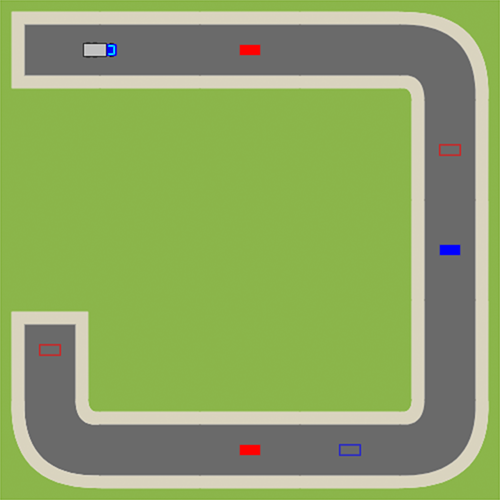
\includegraphics[width=\textwidth]{gfx/exercises-world-d.png}
%     \caption{Beispiel einer Mikrowelt}
%   \end{subfigure}\hfill
%   \begin{subfigure}[b]{0.30\textwidth}
%     \includegraphics[width=\textwidth]{gfx/exercises-program-5.png}
%     \caption{Beispiel eines Programms, welches die Welt löst}
%   \end{subfigure}\hfill
%   \caption{Beispiel Mikrowelt und Minisprache}
% \end{figure}

%************************************************
% Grundlagen
%************************************************
\chapter{Grundlagen}
\label{sec:basics}

In diesem Kapitel werden einige Grundlagen vermittelt, auf welche in späteren Teilen dieser Arbeit verwiesen wird. Aus den Abschnitten "\nameref{sec:basics:playful-learning}" und "\nameref{sec:basics:mini-languages}" werden zudem Anforderungen an diese Arbeit abgeleitet.

%************************************************
% Spielerisches Lernen
%************************************************
\section{Spielerisches Lernen}
\label{sec:basics:playful-learning}

Die im Rahmen dieser Arbeit entwickelte Software soll Lehrer dabei unterstützen, ihren Schülern die Grundlagen des Programmierens zu vermitteln. Dies soll spielerisch geschehen. Prensky führt in seinem Buch \textit{Digital Game-Based Learning} drei Gründe an, warum digitales spielerisches Lernen funktioniert~\cite[147]{prensky2007}:

\begin{enumerate}
    \item Der erste Grund ist das zusätzliche Engagement, das dadurch entsteht, dass das Lernen in einen Spielkontext gebracht wird. Dies kann beträchtlich sein, besonders wenn Menschen nicht lernen wollen.
    \item Der zweite Grund ist der interaktive Lernprozess. Dieser kann und sollte abhängig von den Lernzielen viele verschiedene Formen annehmen.
    \item Der dritte Grund ist die Art und Weise, wie die zwei ersten Gründe im Gesamtpaket zusammengefügt werden. Es gibt viele Möglichkeiten, dies zu tun, und die beste Lösung ist sehr kontextabhängig.
\end{enumerate}

Des Weiteren hängt der Lernerfolg auch immer stark davon ab, wie Spiele vom Lehrer letztendlich eingesetzt werden, aber auch der Stil des Spieles spielt eine Rolle. Damit Spiele -- Lehrspiele im speziellen -- Spaß bringen, müssen sie einige Anforderungen erfüllen. Malone stellt in seinem Artikel \textit{What Makes Computer Games Fun?} eine Checkliste auf, die sich in drei Kategorien gliedert und unter anderem die folgenden Fragen enthält~\cite[49]{malone1981}:

\begin{itemize}
    \item \emph{Herausforderung}: Hat das Spiel ein Ziel? Hat das Spiel einen variablen Schwierigkeitsgrad? Verfügt die Aktivität über mehrere Ziele, z.~B. Zählen von Punkten oder schnelle Reaktionen? Enthält das Programm Zufall? Enthält das Programm versteckte Informationen, die selektiv aufgedeckt werden?
    \item \emph{Fantasie}: Enthält das Programm eine emotional ansprechende Fantasie? Hängt die Fantasie instinktiv mit der in der Aktivität erlernten Fähigkeit zusammen? Ist die Fantasie eine nützliche Metapher?
    \item \emph{Neugierde}: Gibt es audio- und visuelle Effekte, um die Neugier der Sinne zu stimulieren? Gibt es Elemente, die die kognitive Neugier wie Überraschungen oder konstruktives Feedback stimulieren?
\end{itemize}

Diese Anforderungen sollten bei der Aufstellung der Anforderungen für das im Rahmen dieser Arbeit entwickelte Programm berücksichtigt werden, auch wenn sich aufgrund der für diese Art von Lernspiel notwendigen, im nächsten Abschnitt beschriebenen Mechaniken, nicht alle aufgestellten Anforderungen erfüllen lassen werden.

%************************************************
% Minisprachen
%************************************************
\section{Minisprachen}
\label{sec:basics:mini-languages}

Minisprachen sind Programmiersprachen, die speziell auf die Anforderungen von Programmieranfängern zugeschnitten sind, indem sie einen reduzierten Sprachumfang bieten, der speziell auf die Lösung einer bestimmten Klasse von Problemstellungen zugeschnitten ist und dabei die Grundprinzipien des Programmierens hervorhebt bzw. deren Erlernen fördert.

Warum das Erlernen von Programmierfähigkeiten mithilfe von Minisprachen im Gegensatz zu den breit genutzten Universalsprachen (wie z.~B. Java oder C) sinnvoll ist, erklären Brusilovsky et al., indem sie drei Probleme von Universalsprachen für die Anwendung zum Lernen nennen, die Minisprachen zu beheben versuchen \cite[67]{brusilovsky1997}:

\begin{itemize}
    \item Universalsprachen sind zu groß und zu idiosynkratisch. Die konzeptionelle Basis der Sprache bildet zusammen mit den Hauptprinzipien der Programmierung eine große Menge an Material. Anstatt die Grundprinzipien hervorzuheben, rufen die Sprachen nebensächlich Begriffe auf, die die Feinheiten der jeweiligen Sprache und deren Umsetzung, nicht aber die Hauptprinzipien der Programmierung widerspiegeln.
    \item Universalsprachen fördern nicht das Verständnis ihrer grundlegenden Aktionen und Kontrollstrukturen. Die Sprachen sind nicht visuell und ihre Grundfunktionen werden hinter einer undurchsichtigen Barriere ausgeführt. Wenn der Prozess der Programmausführung verborgen ist, entwickelt der Student ein Input-Output-orientiertes Verständnis. Auf diese Weise behindert das Fehlen von visuellem Feedback die Beherrschung der Sprachsemantik.
    \item Da sich Universalsprachen an der Zahlen- und Symbolverarbeitung orientieren, sind die ersten möglichen Aufgaben, die beim Unterrichten der Sprache umgesetzt werden können, weit von den Alltagserfahrungen der Schüler entfernt. Die Entwicklung von Anwendungen, die sowohl informativ als auch interessant sind, erfordert das Erlernen einer beträchtlichen Untermenge der Sprache und das Schreiben recht großer Programme.
\end{itemize}

Brusilovsky et al. heben in Ihrem Artikel \textit{Mini-languages: a way to learn programming principles} einige sich daraus ergebende Eigenschaften von Minisprachen als besonders wichtig hervor \cite[73-74]{brusilovsky1997}:

\begin{itemize}
    \item Sowohl Syntax, als auch Semantik der Sprache sollten \emph{einfach} sein.
    \item Die Operationen der Minisprache sollten \emph{sichtbar} sein. Die meisten Operationen, die der Akteur ausführt, sollten sichtbare Änderungen in der auf dem Bildschirm dargestellten Mikrowelt \TODO{erklären?} vornehmen.
    \item Die Minisprache sollte für die vorgesehene Kategorie von Studenten \emph{attraktiv} und aussagekräftig sein.
    \item Die Sprache sollte \emph{dialogorientiert} sein. Das bedeutet, dass die Sprache Befehl für Befehl in einem Navigationsmodus ausgeführt werden kann (Einzelbefehlsausführung) und als Ganzes in einem Programmiermodus (komplexe Programmausführung).
    \item Die Sprache sollte \emph{modular} sein. Sie sollte einen Mechanismus zum Erstellen abstrakter Anweisungen (Prozeduren) enthalten. Alle Verfahren sollten unabhängige Einheiten sein. Eine solche Prozedur kann als neuer Befehl des Akteurs betrachtet werden, der sowohl im Navigations- als auch im Programmiermodus verwendet werden kann.
\end{itemize}

Aus der Liste dieser Anforderungen ergeben sich direkte Anforderungen an die für diese Arbeit entwickelte Minisprache (siehe \ref{sec:requirements:program}). Sie sind auch -- soweit das beurteilt werden kann -- in allen im nächsten Kapitel genannten vergleichbaren Arbeiten berücksichtigt.

%! Author = Yannick Schröder
%! Date = 17.08.20

%************************************************
% Anforderungsanalyse
%************************************************
\chapter{Anforderungsanalyse}
\label{sec:requirements}

Ziel dieser Arbeit ist die Evaluierung und Migration von GraphQL in die von Marcus Riemer entwickelte Lehr-Entwicklungsumgebung BlattWerkzeug zur Verbesserung des aktuell genutzten Systems.
Nachfolgend wird in diesem Kapitel die Funktionsweise des aktuellen Systems. 
Anschließend werden Anforderungen formuliert und evaluiert die ein neues System größtenteils erfüllen muss.

\section{Aktuelles System}
\label{sec:requirements:system}

Marcus Riemer hat im Rahmen seiner Master-Thesis an der Fachhochschule Wedel die Lehr-Entwicklungsumgebung BlattWerkzeug als Webapplikation entwickelt,
die sich an Kinder und Jugendliche richtet. Mit BlattWerkzeug lassen sich, gestützt durch Drag \& Drop-Edi\-toren,
für beliebige SQLite-Datenbanken Abfragen formulieren und Oberflächen entwickeln~\cite[2]{riemer2016}.
Seit dem Abschluss der Master-Thesis wird BlattWerkzeug im Rahmen eines Promotionsvorhabens weiterentwickelt.

%Server:
Der Server dieser Web-App ist auf Basis von Ruby on Rails gebaut. Er dient hauptsächlich der Speicherung und Auslieferung von Daten.
Kommuniziert wird über eine REST-artige JSON-Schnittstelle~\cite[94]{riemer2016}.

%Client:
Der Client wurde als eine Single-Page Application mit rein clientseitiger Visualisierung aufgebaut,
die lediglich für den Zugriff auf serverseitige Resourcen  (Datenbank, gespeicherte Ressourcen, gerenderte Seiten) Roundtrips zum Server nutzt~\cite[94-95]{riemer2016}.
Programmiert wurde sie 2016~\cite[1]{riemer2016} auf Basis von Angular 2 in TypeScript.
Zum aktuellen Zeitpunkt wird allerdings auf die Angular Version 9.1.0 gesetzt.

%Datenbanksystem
Für die Wahl des einzusetzenden Datenbanksystems wurde sich beim Entwicklungsstart, auf Grund der Kriterien "Kostenlose Verfügbarkeit",
"Einfacher Betrieb", "Einfache Backups", "Tools zur Modellierung" und "Externe Tools zur Entwicklung von SQL-Abfragen"
für eine SQLite Datenbank entschieden~\cite[99-100]{riemer2016}. Im November 2017 ist dann der Grundstein gelegt worden,
um den Server mit einer PostgreSQL Datenbank zu verbinden~\cite{riemerPostgresCommit}, da diese es unter anderem ermöglicht JSON Objekte direkt zu speichern,
ohne diese in Text Datentypen konvertieren zu müssen.

Anhand eines Praxisbeispiels wird im Weiteren die Funktionsweise des Systems in Hinblick auf das Hinzufügen neuer Daten
unter Gewährleistung der Typsicherheit (siehe Unterabschnitt~\fullref{req:typesafe}) verdeutlicht.

\section{Praxisbeispiel - Erweiterung des Datenkonstruktes}
\label{sec:requirements:example}

Damit neue Datensätzen zwischen Server und Client typsicher ausgetauscht werden können sind mehrere Schritte erforderlich.
Die Reihenfolge der nachfolgend aufgeführten Schritte ergibt sich aus dem bisherigen Entwicklungsprozess.

\subsection{Anlegen des Typescript Interfaces}
\label{sec:requirements:example:interface}

Als erstes wird ein Typescript Interface für den Datensatz erstellt, der abgebildet werden soll.
Wir erweitern den Datentyp \emph{Project} aus Listing~\ref{fig:basics:graphql:3} erneut:

\begin{lstlisting}[language=JavaScript,float=h!,caption={Typescript Interface für die Darstellung eines Projektes}, label={lst:example:projectdesc}]
export interface Project {
    id: string;
    name:object;
    public?: boolean;
    slug?: string;
    userId?: string;
    createdAt?: string;
    updatedAt?: string;
}
\end{lstlisting}

\begin{itemize}
    \setlength\itemsep{-1em}
    \item \emph{id/public}: siehe Listing~\ref{fig:basics:graphql:3}.
    \item \emph{name}: hat sich zu einem multilingualen Feld geändert. object repräsentiert den nicht Primitiven Datentyp, also alles was nicht number, string, boolean, symbol, null oder undefined ist~\cite{typescript-object}.
    \item \emph{slug}: ist ein aus einem oder wenigen Wörtern bestehender benutzer- und suchmaschinenfreundlicher
    Text (sprechender Name) als Bestandteil einer URL~\cite{slug-wikipedia}. Diese Angabe ist optional.
    \item \emph{userId}: ist die ID des Nutzers dem dieses \emph{Project} zugeordnet ist (Fremdschlüsselbeziehung).
    \item \emph{createdAt}: ist die optionale zeitliche Angabe wann dieses \emph{Project} erstellt wurde.
    \item \emph{updatedAt}: ist die optionale zeitliche Angabe wann dieses \emph{Project} zuletzt verändert wurde.
\end{itemize}

Wird dieser Datensatz beim Server angefragt, lässt sich die Antwort des Servers auf eine Variable mit dem Typ \emph{Project} zuweisen.
Dadurch wird zur Kompilierzeit ermöglicht typsicher auf die einzelnen Felder des Interfaces zugreifen zu können.

Im nächsten Schritt wird das Interface dem Server zur Verfügung gestellt.

%List Interface/Response Interface
%Dokument Interface
\subsection{Generierung der JSON Schema Definitionen}
\label{sec:requirements:example:schema}
Das Interface aus Listing~\ref{lst:example:projectdesc} wurde clientseitig erstellt und kann auch nur dort verwendet werden. Um es serverseitig nutzen zu können wird daraus eine JSON Schema Datei generiert.
Für die Generierung sind Einträge in einem Makefile nötig, welches sich um die Erstellung aller JSON Schema Dateien, kümmert. Nach der Generierung befinden sich zu jedem aufgeführten Typescript Interface ein passendes JSON Schema in einer eigenen Datei. Diese werden dann in einem Schema Ordner auf Projekt Ebene gehalten. Das jedes Schema in einer eigenen Datei gespeichert ist, kommt dem Server bei der Validierung zu gute. 
Dieser Lädt die Datei, dessen Namen äquivalent zum ursprünglichen Typescript Interface ist, aus dem Ordner, liest das Schema aus und kann dieses zu Validierungszwecken nutzen.

\begin{lstlisting}[float=h!,caption={TypeScript Interface für die Project Darstellung in einer Liste}, label={lst:example:makefile}]
Project.json : $(SRC_PATH)/shared/project.ts
$(CONVERT_COMMAND)
\end{lstlisting}

Mithilfe der JSON Schema Dateien können dann Datensätze validiert werden.

\subsection{Anlegen des Models in Rails}
\label{sec:requirements:example:model}

Sollte das Interface aus Listing~\ref{lst:example:projectdesc} einer neuen Datenbanktabelle entsprechen, muss eine Active Record Migration erstellt werden,
die das Datenbankschema erweitert~\cite{rails-migration}.

\begin{lstlisting}[language=Ruby,float=h!,caption={Rails Migration zum hinzufügen einer \emph{projects} Datenbanktabelle}, label={lst:example:migration}]
create_table "projects", id: :uuid, do |t|
	t.string "slug"
	t.hstore "name", default: {}, null: false
	t.uuid "user_id"
	t.datetime "created_at", null: false
	t.datetime "updated_at", null: false
end
\end{lstlisting}

Durch Ausführung der Migration aus Listing~\ref{lst:example:migration} wird eine neue Tabelle mit der Bezeichnung \emph{projects} erstellt.
Hinzukommend wird ein Active Record Model benötigt, dem die \emph{projects}-Tabelle zugeordnet wird.
Zur Realisierung wird eine Ruby Klasse, die
von der Klasse ApplicationRecord erbt, mit dem selben Namen den die Tabelle hat erstellt.
Die Rails Konvention sieht vor das Datenbanktabellen im Plural und das dazugehörige Model im Singular benannt wird~\cite{rails-naming-convention}.

\begin{lstlisting}[language=Ruby,float=h!,caption={Model}, label={lst:example:model}]
class Project < ApplicationRecord
	# The owner if this project
	belongs_to :user
end
\end{lstlisting}

Auf diese Weise entsteht die Möglichkeit, die Spalten jeder Zeile in dieser Tabelle mit den Attributen der Instanzen des Models abzubilden.
Jede Zeile dieser Tabelle stellt also ein "Projekt" Datensatz mit den in Listing \fullref{sec:requirements:example:interface} aufgeführten Feldern dar.

Um nun auf Anfragen reagieren und Daten aus Model Instanzen an den Client liefern zu können bedarf es einem Controller.

\subsection{Anlegen eines Controllers in Rails}
\label{sec:requirements:example:controller}
Controller haben die Aufgabe Anfragen zu verarbeiten, die vom Router (siehe Listing~\ref{lst:example:router}) an sie weitergeleitet wurden.
Die Funktionen innerhalb eines Controllers sind dafür verantwortlich den Anfragen einen "Sinn" zu geben und die entsprechende Antwort zu erzeugen.
Bei einer Anfrage die Projekt-Daten ausgeliefert bekommen soll, kümmert die Controller Funktion sich darum alle Daten aus dem \emph{Project}-Model
zu holen und gibt diese dann wie bei REST APIs üblich in JSON Form zurück.

\begin{lstlisting}[language=Ruby,float=h!,caption={Route entspricht URL '/project/' und leitet Anfrage an die ProjectsController Funktion \emph{index} weiter }, label={lst:example:router}]
scope 'project' do
	get '/', controller: 'projects', action: :index
end
\end{lstlisting}

\begin{lstlisting}[language=Ruby,float=h!,caption={Controller mit Funktion zum zurückgeben aller Project Instanzen}, label={lst:example:controller}]
class ProjectsController < ApplicationController
	def index
		render json: Project.all
	end
end
\end{lstlisting}

In Zeile 3 des Controllers in Listing~\ref{lst:example:controller} werden um das Beispiel simpel alle Projekte aus der Datenbank geladen und in JSON Form
zurück gegeben. Im aktuellen System hingegen werden die Projekte paginiert an den Client geliefert, damit nicht aus Versehen riesige Datensätze an den Client übertragen werden. Um gewährleisten zu können, das die Antwort vom Server auch die erwarteten Daten liefert, wird ein
Test geschrieben der prüft, ob die Antwort dem clientseitig erstellten Interface aus Listing~\ref{lst:example:projectdesc} entspricht.
Für die Validierung wird ein für Ruby entwickelter JSON Schema Validator genutzt.

\begin{lstlisting}[language=Ruby,float=h!,caption={Test überprüft, ob bei Anfrage der Route '/project/' eine Antwort vom Typ Project folgt}, label={lst:example:controller-test}]
it 'lists a single project' do
	FactoryBot.create(:project, :public)
	get "/project/"
	
	expect(response).to have_http_status(200)

	parsed = JSON.parse(response.body)
	expect(parsed['data'].length).to eq 1

	# Validierung gegen  das "Project" interface
	expect(parsed['data'][0]).to validate_against "Project"
end
\end{lstlisting}


\begin{itemize}
	\setlength\itemsep{-1em}
	\item \emph{Zeile 2}: Erstellt eine \emph{Project} Instanz und speichert diese in der Datenbank.
	\item \emph{Zeile 3}: Ein GET Request wird an die Route "/project/" geschickt.
	\item \emph{Zeile 5}: Es wird der HTTP Status 200 erwartet. 
	\item \emph{Zeile 7}: Parst den response body in JSON.
	\item \emph{Zeile 8}: Erwartet das die Länge der empfangenen Datensätze 1 ist.
	\item \emph{Zeile 11}: Validiert die Antwort gegen das JSON Schema \emph{Project}.
\end{itemize}

Der Server hat nun die Fähigkeit auf eine Anfrage nach allen Projekten zu reagieren.
Somit muss der Client noch die Möglichkeit erhalten eine Anfrage zu erstellen und die Antwort grafisch abbilden zu können.

%Für jede Sicht (z.B. Admin/Frontend) eine Route und Controller Funktion.
\subsection{Dataservices auf dem Client}
\label{sec:requirements:example:service}
In der Welt von Angular gibt es eine strikte Trennung zwischen Darstellung und Verarbeitung von Daten~\cite{angular-service}.
Für die Verarbeitung von Daten, wie das Abrufen, werden Angular Services genutzt. Diese sind typischerweise Typescript Klassen,
deren Verwendungszwecke genau definiert sind. Der im Folgenden beschriebene Service hat die Aufgabe Projekt-Daten zu verarbeiten.

\begin{lstlisting}[language=JavaScript,float=h!,caption={Funktion zum Abruf aller Projekte vom Server}, label={lst:example:service}]
@Injectable()
export class ProjectsDataService {
    constructor(private http: HttpClient) { }
    // Die Antwort soll dem Typparameter "Project" entsprechen
    readonly projects = this.http.get<Project>('/project/');
}
\end{lstlisting}

\begin{itemize}
    \setlength\itemsep{-1em}
    \item \emph{Zeile 1}: \emph{@Injectable} stellt sicher, dass der Compiler die notwendigen Metadaten erzeugt, um die Abhängigkeiten der Klasse zu erstellen, wenn die Klasse injiziert wird.
    \item \emph{Zeile 2}: Deklarierung der Klasse/des Services ProjectsDataService
    \item \emph{Zeile 3}: Injizierung des HttpClient~\cite{angular-http} in den Service
    \item \emph{Zeile 5}: Nutzung des HttpClient zur Erstellung eines typisierten HTTP-Requests, welcher zur bereits hinzugefügten Route in Listing~\ref{lst:example:router} führt.
    Dieser wird auf die readonly Variable projects geschrieben.
\end{itemize}

Hinzuzufügen ist, das dieses Beispiel nur bedingt dem aktuellen System entspricht, da im eigentlich eine einheitliche Service Klasse mit einem Cache verwendet wird, von der der ProjectsDataService erbt. Das Aufzeigen der einheitlichen Service Klasse würde jedoch den Rahmen sprengen.

Die Angabe des Antworttyps \emph{Project} in Zeile 5 fungiert dabei zur Kompilierungszeit als Type Assertion~\cite{typescript-typeassertion}
und erleichtert den Zugriff auf die Attribute der Antwort. Der TypeScript Compiler führt während der Laufzeit jedoch keine Überprüfung durch.
Er geht an dieser Stelle davon aus, das der Entwickler spezielle Prüfungen, wie z.B. der Test in Listing~\ref{lst:example:controller-test}, durchgeführt hat.

Die Dartsellung der erhaltenen Daten übernehmen dann Angular Komponenten, in die Services "injiziert" werden können.
Dadurch können Komponenten die Funktionen eines injizierten Services nach Belieben nutzen.

\subsection{Komponenten auf dem Client}
\label{sec:requirements:example:component}

Eine Angular Komponente entspricht einem Teilbaum des DOM-Baums, auch View genannt.
Somit wird eine Komponente für einen bestimmten Zweck erstellt,
der in unserem Fall die grafische Auflistung der Projekt-Daten ist.

\begin{lstlisting}[language=JavaScript,float=h!,caption={Funktion zum Abruf aller Projekte vom Server}, label={lst:example:component}]
@Component({
    selector: "project-list",
    templateUrl: "templates/project-list.html",
})
export class ProjectListComponent {
    // Injizierung des ProjectsDataService
    constructor(private _projectsData: ProjectsDataService) {}

    readonly projects = this._projectsData.projects;
}
\end{lstlisting}

\begin{itemize}
    \setlength\itemsep{-1em}
    \item \emph{Zeile 1}: Annotierung einer Typescript-Klasse als Komponente.
    \item \emph{Zeile 2}: Der Wert von \emph{selector} kann als HTML-Tag (<project-list></project-list>) in Templates genutzt werden,
    um diese Komponente Instanziieren und das zugehörige Template innerhalb des Bezeichners rendern zu können.
    \item \emph{Zeile 3}: Festlegung des Pfades, wo sich das zu rendernde Template, also der darzustellende HTML Code befindet.
    \item \emph{Zeile 5}: Deklarierung der Klasse/des Komponente ProjectListComponent.
    \item \emph{Zeile 7}: Injizierung des ProjectsDataService~\cite{angular-http} in die Komponente.
    \item \emph{Zeile 9}: Speichern der Funktion aus dem ProjectsDataService zum Abrufen der Projekt-Daten auf eine Instanzvariable.
\end{itemize}

Eine Komponente stellt HTML Code dar, der in einer Datei gespeichert wird, die als Template bezeichnet wird.
Innerhalb des Templates ist der Zugriff auf die nicht privaten Variablen der Komponenten gegeben.
Das zugehörige Template project-list.html sieht folgendermaßen aus:

\begin{lstlisting}[language=JavaScript,float=h!,caption={Funktion zum Abruf aller Projekte vom Server}, label={lst:example:service}]
<project-list-item
  *ngFor="let project of projects | async"
  [project]="project"
></project-list-item>
\end{lstlisting}

\begin{itemize}
    \setlength\itemsep{-1em}
    \item \emph{Zeile 1}: Aufruf der Komponente mit dem \emph{selector} "project-list-item".
    Diese übernimmt hier die Darstellung eines einzelnen Projektes innerhalb einer Liste und verdeutlicht damit
    die Modularität von Angular Komponenten.
    \item \emph{Zeile 2}: *ngFor ist die "Repeater"-Direktive ~\cite{ng-for} in Angular.
    Sie ermöglicht ein gegebenes HTML Template einmal für jeden Wert in einem Array zu wiederholen,
    wobei jedes Mal der Array-Wert als Kontext übergeben wird. Das Array \emph{projects} kommt aus der Komponenten in Listing~\ref{lst:example:component} Zeile 9.
    \item \emph{Zeile 3}: Übergibt den Wert aus dem Array an eine mit \emph{@Input()} annotierte Variable \emph{project} aus der "project-list-item" Komponenten.
\end{itemize}

Diese Schritte sind in ihrer Gänze nur bei der Einführung neuer Entitäten notwendig.
Bei der Nutzung von Subtypen kann ein Teil der umgesetzten Schritte wiederverwendet werden,
bzw ist nur einmal erforderlich gewesen, wie das Ausführen einer Datenbankmigration.

\subsection{Anlegen einer neuen Sicht}
\label{sec:requirements:example:newview}

Für das Bereitstellen einer neuen Sicht auf die Projekt Daten sind mehrere Schritte zu wiederholen (siehe Tabelle~\ref{tbl:newview}).

\begin{table}[h!]
    \begin{tabular}{|p{0.12\textwidth}|p{0.52\textwidth}|p{0.12\textwidth}|}
        \hline
        \textbf{Schritt} & \textbf{Beschreibung} & \textbf{Aktuelles \newline System} \\ \hline
        $\ref{sec:requirements:example:interface}$ & Anlegen eines Interfaces & $\surd$  \\ \hline
        $\ref{sec:requirements:example:schema}$ & Eintrag in Makefile & $\surd$\\ \hline
        \multirow{2}{*}{$\ref{sec:requirements:example:model}$}
        & Anlegen einer Datenbank Migration & $X$  \\
        & Anlegen des Models & $X$ \\ \hline
        \multirow{4}{*}{$\ref{sec:requirements:example:controller}$}
        & Route definieren & $\surd$  \\
        & Anlegen des Controllers & $X$  \\
        & Controller Funktion schreiben & $\surd$  \\
        & Tests schreiben & $\surd$  \\ \hline
        \multirow{2}{*}{$\ref{sec:requirements:example:service}$}
        & Anlegen eines Angular Services & $X$  \\
        & Funktion zum Abschicken einer Query & $\surd$  \\ \hline
        \multirow{2}{*}{$\ref{sec:requirements:example:component}$}
        & Anlegen einer Angular Komponenten & $\surd$  \\
        & Anlegen eines Templates & $\surd$  \\ \hline
    \end{tabular}
    \vspace{5pt}
    \centering
    \caption{Vergleich der Funktionweise des aktuellen Systems mit GraphQL in Bezug auf die Erstellung neuer Sichten auf bereits vorhandene Datensätze}
    \label{tbl:newview}
\end{table}

Auffallend ist, dass im aktuellen System 8 von 12 Schritte erneut ausgeführt werden müssen.

\section{Vorteile des bisherigen Ansatzes}
\label{sec:requirements:pros}
Die Verwendung des derzeitigen Systems hat viele Vorteile,
deren Gewichtung in Hinsicht auf die Migration eines neuen Systems zu evaluieren gilt.
Nachfolgend werden die wichtigen Vorteile erläutert.

\subsection{Typescript Typsystem}
\label{sec:requirements:pros:typescript}
Ein Vorteil ist die Verwendung des umfangreichen Typescript Typsystems.
Dieses ermöglicht neben Typüberprüfungen zur Kompilierzeit auch Vererbungen zwischen Interfaces, die Abbildung verschiedenster Typvarianten wie
Union Types, zur ermöglichung verschiedener Typen innerhalb einer Variablen, Intersection Types zum zusammenfügen von Typen,
Generische Typen, sowie Utility Types um bestehende Typen zu manipulieren.
In Abschnitt~\fullref{sec:basics:typescript} wurden bereits mehrere Möglichkeiten dazu vorgestellt.

\subsection{Typescript zu JSON Schema Generatoren}
\label{sec:requirements:pros:generation}
Hinzukommend können "Typescript zu JSON Schema Generatoren" Annotationen innerhalb der Typescript Interfaces verarbeiten~\cite{json-schema-generator-annotations}.
Dadurch können Wertebereiche vorgegeben bzw. eingeschränkt werden,
wie das Setzen eines Minimums bzw. Maximums bei Zahlen, die Verwendung von Reguläre Ausdrücke für Zeichenketten,
die Angabe wie viele Elemente ein Array minimal bzw. maximal aufnehmen kann,
so wie die Angabe wieviele Attribute ein Objekt minimal bzw. maximal haben darf und welche erwartet werden.
Zudem ermöglichen die Generatoren die Bereitstellung der clientseitig erstellten Typdefinitionen in Form von JSON Schema Dateien.

\subsection{Modularität}
\label{sec:requirements:pros:modul}
Aus Unterabschnitt~\fullref{sec:requirements:pros:generation} ergibt sich eine bessere Modularität.
Der Kern des Systems zur typsicheren Kommunikation besteht aus den drei Punkten Typescript Interface, Typescript zu JSON Schema Generator und
JSON Schema Validator. Die ersten beiden Punkte sind unabhängig vom Backend.
Zudem sind JSON Schema Validatoren in 19 Sprachen~\cite{json-schema-implementations} bereitgestellt worden, wodurch das Backend austauschbar ist.
Daher kann der Client auch mit anderen APIs typsicher kommunizieren, wenn diese Zugriff auf dessen Typdefinitionen erhalten.

\subsection{Typsicherheit zur Kompilierzeit}
\label{sec:requirements:pros:typesafe-compile}
Im Client sorgt das Typescript Typsystem durch für Typsicherheit zur Kompilierzeit.

Typsicherheit auf dem Server stellt sich schwieriger dar. In der Welt von Ruby wird nur mit Objekten ohne Typangabe gearbeitet.
Auf eine Variable in der eine Zeichenkette steckt, kann z.B. eine Zahl zugewiesen werden. Wenn anschließend eine Funktion der String Klasse
im guten Glauben das es sich bei der Variablen noch um eine Zeichenkette handelt, auf einer Zahl aufgerufen wird, kommt es zu einem Laufzeitfehler.
Ein ausreichendes Sicherheitsgefühl wurde dennoch durch umfangreiches Testen der Controller, Models und Helper erlangt.

Ungeachtet dessen besteht das Problem, dass zur Laufzeit eingehende Daten ungewollte Beschaffenheiten aufweisen können.

\subsection{Typsicherheit zur Laufzeit}
\label{sec:requirements:pros:typesafe-runtime}
Beim Kompilieren von Typescript zu Javascript werden alle Typinformationen entfernt.
Wenn also Daten von einer Schnittstelle abgerufen werden, kann nicht sichergestellt werden das diese korrekt ankommen, woraus
ungewolltes Verhalten resultieren kann.

Um ungewolltem Verhalten vorzubeugen wurden Fehlerbehandlungen hinzugefügt, bei denen jede Anfrage auf Korrektheit geprüft wird.
Voraussetzung ist, dass eigehende Anfragen gegen den selben Typen validiert werden,
den der Client für das Abschicken nutzt und dieser Typ bei Anfragen zum Erstellen oder Ändern von Daten kompatibel mit dem Datenbankschema ist.
Hinzuzufügen ist das wie in Abschnitt~\ref{sec:requirements:example:schema} beschrieben, aus Interfaces JSON Schema Dateien erzeugt werden,
die für die Validierung vom JSON Schemer Validator gebraucht werden. Somit wird indirekt gegen die Typescript Interfaces validiert.

Zusätzlich wurden auf dem Server Request Specs genutzt.
Diese können zur Kompilierzeit Laufzeitfehler in der API Kommunikation bestmöglich ausschließen.
Sie Testen das Verhalten der Controller, durch abschicken von HTTP-Requests und prüfen, ob die Antwort die erwartete Beschaffenheit ausweist. 

Diese Tests wurden in den Deployment Prozess der Webapplikation eingebaut. Bei fehlgeschlagen einiger Tests wird die Bereitstellung der Software
verhindert, wodurch zur Laufzeit ein typsicheres Verhalten suggeriert wird.

\begin{figure}[h!]
    \centering
    \includegraphics[width=\linewidth]{snippets/server-client-api.pdf}
    \caption{Typsichere Kommunikation zwischen Typescript Client und Ruby Server}
    \label{req:typesafe:server-client-short}
\end{figure}

\subsection{Stabilität}
\label{sec:requirements:pros:stable}
Die Software Blattwerkzeug ist seit mehreren Jahren in der Entwicklung. Von Beginn an (2016) wird
eine REST-artige JSON-Schnittstelle verwendet (siehe Kapitel 4.1. Client-Server-Architektur ~\cite{riemer2016}).
Im laufe der Zeit wurden viele Tests entwickelt die sicher stellen das alles wie erwartet funktioniert.
Somit hat sich das aktuelle System seit mehreren Jahren bewährt.

\section{Nachteile des bisherigen Ansatzes}
\label{sec:requirements:cons:typescript}
Auch wenn ein System funktionstüchtig ist, ist es nicht zwangsläufig perfekt.
In diesem Abschnitt werden die relevanten Nachteile der bisherigen Umsetzung ausgearbeitet.

\subsection{Manuelle SQL Queries}
Für alle im Client darzustellenden Models müssen die zwei Funktionen \lstinline|to_full_api_response| und \lstinline|to_list_api_response| entwickelt werden.
\lstinline|to_full_api_response| selektiert alle Attribute die ein Admin sehen darf. Nur ein Teil dieser Attribute wird im Admin Bereich auch wirklich gebraucht, sie sollen trotzdem dem Admin zugängig gemacht werden.
\lstinline|to_list_api_response| selektiert nur die Attribute die ein normaler Nutzer sehen darf. Dieses Verfahren ist sehr unflexibel und wird schnell aufwendig wenn noch weitere Rollen dazu kommen mit anderen Berechtigungen in Bezug auf das Anzeigen von Daten.
%\subsection{Ruby ohne Typangaben}
%Umfangreiches Testen von untypisiertem Rubycode kann zwar das Gefühl von Sicherheit vermitteln, %dieses hängt allerdings von der Fähigkeit des Programmierers ab, alle möglich Fälle die eintreten %können mit den Tests abzudecken.
%rest-projects-list-huge.png
%Eine alternative Idee dazu wäre die Nutzung eines von vielen Rubygems wie %\emph{typesafe-ruby}~\cite{typesafe-ruby}
%oder \emph{sorbet}~\cite{sorbet} die versprechen Rubycode typsicher zu machen. Diese Tools werden %sich im aktuellen System nicht zu Nutze gemacht.

\subsection{Auswahl von Attributen}
\label{sec:requirements:cons:attributes}
Bei allen im Kontext dieser Arbeit relevanten Listendarstellungen im Client treten Overfetching Probleme auf.
Die Listendarstellung von Projekten im Admin Bereich werden 3 von 11 Attributen in der Liste angezeigt. 
Um dies als Nachteil zu untermauern, wird die Größe des im aktuellen System übertragenen JSON Objektes (siehe Abbildung~\ref{req:rest-projects-list-huge}) mit einem JSON Objekt verglichen, welches nur die 3 anzuzeigenden Attribute der Projektdaten beinhaltet (siehe Abbildung~\ref{req:rest-projects-list-small}). Die Größe eines Objektes ohne überflüssige Attribute, ist bei einer Listengröße von 5 Projekten fast 5 mal kleiner.
Bei den beiden Abbildungen handelt es sich um Screenshots aus dem Firefox Netzwerkanalyse Tool.

\begin{figure}[h!]
	\centering
	\includegraphics[width=\linewidth]{snippets/rest-projects-list-small.png}
	\caption{Anfrage der Projekt Liste und Antwort mit nur den 3 anzuzeigenden Attributen}
	\label{req:rest-projects-list-small}
\end{figure}

\begin{figure}[h!]
	\centering
	\includegraphics[width=\linewidth]{snippets/rest-projects-list-huge.png}
	\caption{Anfrage der Projekt Liste und Antwort mit allen Attributen}
	\label{req:rest-projects-list-huge}
\end{figure}

Möchte man zusätzlich noch Beziehungen abbilden kann ebenfalls das in Abschnitt~\fullref{sec:basics:restapi:interface} beschriebene Underfetching Problem auftauchen.
Dieses ließe sich im aktuellen System durch manuelle Erstellung der SQL Queries beheben.

\subsection{Camel Case und Snake Case Notationen}
Da in Ruby für Benennungen von Variablen, Methoden, Dateien etc. Snake Case und auf dem Typescript Client Camel Case verwendet wird, müssen Datensätze nach auslesen aus der Datenbank vor dem Ausliefern an den Client zu Camel Case konvertiert werden. Das gleiche gilt wenn Anfragen zum Erstellen von Datensätzen an den Server geschickt werden. Bevor diese in die Datenbank eingefügt werden können, muss die Schreibweise der einzelnen Attribute zu Snake Case verändert werden.

\subsection{Am Rande der Skalierbarkeit}
Die Haltung der zur JSON Schema Generierung benötigten Informationen zu jedem Interface - Pfad der Datei, Name des Interfaces, Name der generierten Zieldatei -
in einem Makefile ist unübersichtlich und deren Eintragung kann leicht vergessen werden. 
Ein weiterer Nachteil und Einschränkung des Entwicklers ist der Programmieraufwand bei der Erstellung neuer Abfragen bzw. neuer Sichten (siehe Tabelle~\ref{sec:requirements:example:newview}).
So wie das System aktuell ist skaliert es noch ausreichend. Je größer allerdings die Anwendung wird, je mehr generierte Typen verwendet werden und je mehr unterschiedliche Sichten gebraucht werden desto schlechter skaliert es.

\section{Anforderungen}
\label{sec:requirements:req}
In diesem Abschnitt sind Kernanforderungen an ein neues System formuliert.
Aus dem Abschnitt~\fullref{sec:requirements:system} konnten sich bereits mehrere dieser Anforderungen ableiten lassen.

\subsection{Darstellungsvielfalt}
\label{sec:requirements:req:view}
Als erste Anforderung wird die Darstellungsvielfalt definiert.
In einer Webapplikation, in der Nutzer verschiedene Rollen zugewiesen bekommen, wodurch sie Berechtigungen erhalten,
werden je nach Rolle unterschiedliche Funktionalitäten und Sichten auf Daten gewährt.

Im aktuellen System wird zwischen den Rollen Admin, Owner und User unterschieden - beschrieben in Kapitel 3.2.6 Rollen und Autorisierung
in der Abschlussarbeit von Tom Hilge~\cite{Abschlussarbeit-Tom-Hilge}.
Die relevanten Berechtigungen der einzelnen Rollen sind in Tabelle~\ref{tbl:req:roles} beschrieben.

\begin{table}[h!]
    \begin{tabular}{|p{0.34\textwidth}|p{0.3\textwidth}|p{0.08\textwidth}|p{0.08\textwidth}|p{0.08\textwidth}|}
        \hline
        \textbf{Berechtigung} & \textbf{Beschreibung} & \textbf{Admin} & \textbf{Owner} & \textbf{User} \\ \hline
        \multirow{3}{*}{Sichten im Frontpage Bereich}
        & Projekt Liste & $\surd$ & $\surd$ & $\surd$\\
        & Projekt Details & $\surd$ & $\surd$ & $\surd$\\
        & Projekt Erstellen & $\surd$ & $\surd$ & $\surd$ \\
        \hline
        \multirow{2}{*}{Sichten im Admin Bereich}
        & Erweiterte Projekt Liste & $\surd$ & $X$ & $X$\\
        & Erweiterte Projekt Details & $\surd$ & $X$ & $X$\\
        \hline
        \multirow{1}{*}{Geplante Sichten}
        & Projekt Liste eines Owners & $\surd$ & $\surd$ & $X$\\
        \hline
    \end{tabular}
    \vspace{5pt}
    \caption{Zugriffsberechtigungen auf Projekt Daten der verschiedenen Rollen zur Hervorhebung der benötigten Darstellungsvielhalt}
    \label{tbl:req:roles}
\end{table}

Viele dieser Sichten nutzen unterschiedliche Subtypen des Projekttypen.
Beispielsweise listet die Projektliste auf der Frontpage nur öffentliche Projekte - bei denen das Attribut \emph{public} auf \emph{true} gesetzt ist -
auf und zeigt dabei die Datenfelder "name", "description", "slug" und "defaultProgrammingLanguage" an.
Die Projektliste im Adminbereich zeigt im Gegensatz dazu alle Projekte an und greift auf
die Datenfelder "name", "slug", "Anzahl der Code Ressourcen" und die "id" zu.
Die Bedeutung der Felder "defaultProgrammingLanguage" und "Anzahl der Code Ressourcen" ist in diesem Kontext irrelevant und wird nicht näher erläutert.

Zu diesen unterschiedlichen Sichten kommen noch Weitere Spezifikationen in der Dartsellung die gefordert sind.

\subsubsection{Mehrsprachigkeit}
Die Webapplikation von Marcus wird aktuell in zwei Sprachen Angeboten, Deutsch und Englisch.
In Abbildung~\fullref{fig:basics:graphql:6} wurde bereits suggeriert das das Feld \emph{name} eines Projektes nach Sprachen gefiltert werden kann.
Bislang wurde \emph{name} als reiner string behandelt (siehe Listing~\ref{lst:example:projectdesc}). Im aktuellen System werden Mehrsprachige Felder
als hstore (Hash mit Tiefe 1) in der Datenbank gehalten. Der Schlüssel gibt den zweistelligen Ländercode nach ISO Alpha-2 \cite{iso-alpha-2} an
und der dazugehörige Wert den Namen des Projektes in der jeweiligen Sprache.

\begin{lstlisting}[language=JavaScript,float=h!,caption={Speicherung der Projektnamen als jsonb}, label={sec:requirements:multilang}]
{
    "de"=>"Drei Fragezeichen",
    "en"=>"Three Investigators"
}
\end{lstlisting}

Das Sprachenangebot gilt bei einer Systemmigration weiterhin als gefordert und soll zukünftig erweiterbar sein.

\subsubsection{Sortieren und Paginierung}
Die Paginierung ist das Portionieren großer Datensätze zur übersichtlicheren und schnelleren Verarbeitung und Darstellung.
In Blattwerkzeug werden alle Listenansichten im Admin Bereich in einer Tabelle paginiert angezeigt.
Ein Datensatz der einer Liste mit 30 Einträgen entspricht würde bei einer Paginierung mit der Seitengröße 5 auf 6 Seiten aufgeteilt werden.
Ein Menü zum traversieren der Einträge könnte wie in Listing~\ref{req:view:pagination} aussehen.

\begin{figure}[h!]
    \centering
    \includegraphics[width=\linewidth]{snippets/paginierung.pdf}
    \caption{Menüleiste zum Wechseln der Seite und Einstellen der Seitengröße}
    \label{req:view:pagination}
\end{figure}

Hinzukommend soll es möglich sein eine Liste nach verschiedenen Attributen sortieren zu können, auch wenn diese mehrsprachig sind und
in der Datenbank als hstore (siehe Abschnitt~\ref{sec:basics:postgres}) gespeichert werden.

\subsubsection{Filtern}

Für Listendarstellungen soll es möglich serverseitig Einträge effizient, also möglichst direkt in SQL zu filtern.


\subsection{Typdefinitionen}

Typdefinitionen (als Ganzes Typschema genannt) sind die Grundlagen für typsichere Webapplikationen.

Gefordert wird, dass sowohl serverseitige, als auch clientseitige Applikationen sich ein Typschema teilen. 
Die Alternative, dass jede Applikation ein eigenes Typschema hält ist keine Option. Diese müssten mit viel Aufwand zu jedem Zeitpunkt synchron gehalten werden, wodurch bei jeder Änderung eines Schemas alle Weiteren angefasst werden müssten. Dies würde keine Verbesserung zum aktuellen System bedeuten.

Somit muss ein Typschema, wie in Listing~\fullref{req:typesafe} erwähnt, systemübergreifend zur Verfügung gestellt werden.

\subsubsection{Übersetzung des Typschema durch Codegenerierung}
Codegeneratoren ermöglichen das Übersetzen eines Typschemas in ein Anderes, wie z.B. von Typescript zu JSON Schema.
Sie sind für die zentrale Haltung und Nutzung nur eines Typschemas ausschlaggebend.

Gefordert ist bei der Einführung eines Typschemas, das entsprechende Generatoren für alle angebundenen Applikationen vorhanden sind.

\subsubsection{Datenbankschema}
Zusätzlich wird gefordert, dass das Typschema mit dem bereits vorhandenen Datenbankschema kompatibel ist.
Bei Abweichungen, wie der Speicherung eines Datums in verschiedenen Datumsformaten,
werden Übersetzungen nach auslesen oder vor dem Einfügen in die Datenbank gefordert.

Codegeneratoren können hierbei nur in eine Richtung genutzt werden.
Diese bezieht sich auf die Generierung von Typen aus dem Datenbankschema zum Beispiel mithilfe des Rubygems \emph{schema2type}~\cite{schema2type}.

Die Generierung eines Datenbankschemas aus Typdefinitionen ist nicht zu empfehlen.
Zum einen muss für jeden Typen angegeben werden, ob dieser eine Datenbanktabelle darstellt oder z.B. nur ein Subtyp ist.
Zum anderen sind komplexe Beziehungen zwischen Typen schwer abzubilden.

Also ist mit einer Koexistenz zwischen zentralem Typschema und Datenbankschema zu rechnen.

\subsubsection{Synchronisation der Typdefinitionen}
Sollte das zentrale Typschema für eine Applikation übersetzt werden,
müssen das übersetzte Schema synchron zum Ursprünglichen bleiben. Dies sollte in den Prozess der Bereitstellung der Software eingebunden werden.

Ein neues System muss also folgende Anforderungen erfüllen:

\begin{itemize}
    \setlength\itemsep{-1em}
    \item Zentrales Typschema
    \item Übersetzung des Typschemas für jede Applikation
    \item Synchronität aller Schemata
    \item Kompatibilität mit Datenbankschema
\end{itemize}

\subsection{Typsicherheit}
\label{req:typesafe}
Eine weitere grundlegende Anforderung bei der Entwicklung einer Webapplikation ist die Typsicherheit.
Im Kontext der Arbeit werden Typsicherheit auf dem Client,
dem Server und die typsichere Kommunikation zwischen Client und Server miteinander in Bezug gebracht.
Sind die drei Punkte gegeben wird von einer Typsicheren Webapplikation gesprochen.

\subsubsection{Auf dem Client und Server}
\label{req:typesafe:client}
Die Typsicherheit ist im aktuellen System clientseitig und serverseitig ausreichend gegeben (siehe Unterabschnitt~\fullref{sec:requirements:pros:typesafe-compile} und Unterabschnitt~\fullref{sec:requirements:pros:typesafe-runtime}).
Es wird mindestens gefordert das sich diese mit Einführung eines neuen Systems nicht verschlechtert.

\subsubsection{Kommunikation zwischen Server und Client}
\label{req:typesafe:api}
Während des Datenaustausches zwischen Client und Server kann es durch fehlerhafte Daten zu Laufzeitfehlern kommen.
%Diese sind in einer Webapplikation sehr unschön, da außer bei einer fehlerhaften Eingabe in Formularen, dem Nutzer
%meist lediglich gezeigt wird das etwas schief gelaufen ist, dieser aber keine Möglichkeit zur Fehlerbehebung erhält.

Dieses Problem lässt sich bei eingehenden Daten durch Validierungen jeder Anfrage und Antwort auf ihre Korrektheit lösen.
Vorausgesetzt ist, dass jede eingehende Anfrage gegen den \textbf{selben} Typen validiert wird,
den der Client auch für das Abschicken nutzt und kompatibel mit dem Datenbankschema ist.
Umgekehrt gilt, dass jede Antwort gegen den selben Typen serverseitig validiert wird, den der Client zur Speicherung der Antwort verwendet.
Voraussetzung dafür sind systemübergreifende Typdefinitionen, in Abbildung~\ref{req:typesafe:server-client-short} SCHEMA genannt.

Die folgenden Beispiele zeigen in welchem Ausmaß die Validierung der Daten gefordert ist. In Abbildung~\ref{req:typesafe:request-validation} wird durch ein Formular die Erstellung eines Projektes demonstriert. Die Inhalte des Formulars werden auf ein Objekt vom Typ \emph{CreateProjekt} (siehe Listing~\ref{req:typesafe:createproject}) geschrieben und an den Server geschickt. Dort wird der eingehende Datensatz gegen den selben Typ validiert. Treten hierbei Fehler auf, wird der Datensatz nicht in die Datenbank geschrieben und der HTTP Status 400 zurück gegeben.
Wird der Datensatz erfolgreich validiert, wird der Datensatz in der Datenbank gespeichert und der HTTP Status 200 an den Client geschickt.

\begin{lstlisting}[language=Javascript,float=h!,caption={Interface zum Erstellen eines Projektes}, label={req:typesafe:createproject}]
interface CreateProject {
  name: string;
  slug?: string;
  public: boolean;
}
\end{lstlisting}

\begin{figure}[h!]
	\centering
	\includegraphics[width=\linewidth]{snippets/project-create-validation.pdf}
	\caption{Validierung von Requests zum Erstellen eines neuen Projekt Datensatzes}
	\label{req:typesafe:request-validation}
\end{figure}

In Abbildung~\ref{req:typesafe:list-validation} wird eine Liste von Projekten deren Attribut \emph{public} auf \emph{true} gesetzt ist beim Server angefragt. Bevor diese Liste an den Client zurück gegeben wird, wird gefordert, dass diese gegen das Interface validiert wird, welches der Client zur Darstellung nutzt (siehe Listing~\ref{req:typesafe:listproject}). Schlägt die Validierung fehl, wird der HTTP Status 400 zurück gegeben, ansonsten der Datensatz (inkl. HTTP Status 200).

\begin{lstlisting}[language=Javascript,float=h!,caption={Interface zum Auflisten von Projekten}, label={req:typesafe:listproject}]
interface ListProject {
  id: string;
  name: string;
  slug?: string;
}
\end{lstlisting}

\begin{figure}[h!]
    \centering
    \includegraphics[width=\linewidth]{snippets/project-list-validation.pdf}
    \caption{Validierung von Responses zum Auflisten von Projekt Datensätzen}
    \label{req:typesafe:list-validation}
\end{figure}

Ein neues System muss als Anforderung mindestens den aktuellen Grad an Sicherheit aufweisen durch:

\begin{itemize}
    \setlength\itemsep{-1em}
    \item Systemübergreifendes Validieren gegen die selben Typen
    \item Validierung von Anfragen
    \item Validierung von Antworten
    \item Testen der Schnittstellen, um Laufzeitfehler vorzubeugen.
\end{itemize}

%Erfordert applikationsübergreifende Typdefinitionen.
%JSON Schema Validator für Datenbankfelder:
%/models/json schema validator
%JSON Schema Validator für Requests:
%grammars controller update
%JSON Schema Validator für Responses:
%Rspec
%JSON Schema Erzeugung aus Typescript Interfaces:
%Aktuell werden Clientseitig JSON Schema Dateien mithilfe von Typescript Interfaces und einem ellenlangen Makefile generiert.

\subsection{Performance und Skalierbarkeit}
Performanz und Skalierbarkeit sind bei der Wahl eines Systems ausschlaggebende Kriterien. Das aktuelle System weist im Bereich der Kommunikation Schwächen auf, die es zu Beheben gilt.

\subsubsection{Over- und Underfetching}
Over- und Underfetching sind für eine REST API typische Probleme.
In Unterabschnitt~\fullref{sec:requirements:cons:attributes} wurde bereits gezeigt weshalb diese ein Nachteil in der Performanz darstellen.
Ein neues System sollte diese Probleme beheben können.
Wichtig ist, dass nicht für jede gekürzte Sicht ein Subtyp und eine neue Route inkl. Controllerfunktion erstellt wird. Des weiteren dürfen Beziehungen zwischen Daten nicht das Abfeuern übermäßig vieler Requests bedeuten.

\subsubsection{N+1 Query Problem}
Ein Weiterer Aspekt der die Performanz und Skalierbarkeit einschränkt ist das N+1 Query Problem bei Datenbankabfragen. Dieses unterscheidet sich kaum zu dem bereits erwähnten N+1 Query Problem bei Abfragen an die Web API. Beide Beschreiben einen Engpass der bei Hochskalierung von Anfragen zu Einbußen in der Performanz führt. 

Datenbankabfragen werden auch nach der Migration eines neuen Server Roundtrip Verfahrens serverseitig von Rails ausgeführt. Wurde das N+1 Query Problem beim Anfrage der Web API gelöst, kann es dennoch zum Abschicken von N+1 Datenbankabfragen kommen.

Dieses Problem gilt als Anforderung zu lösen.

\subsubsection{Cache}
Die Nutzung eines Caches soll bei HTTP Anfragen bereitgestellt werden.
TODO: Weiter ausführen, aber kurz halten


\begin{itemize}
	\setlength\itemsep{-1em}
	\item Lieferung nur benötigter Daten
	\item Abschicken möglichst weniger Anfragen an die Web API
	\item Abschicken möglichst weniger Anfragen an die Datenbank
	\item Möglichkeit zur Nutzung eines Caches
\end{itemize}

\subsection{Validierung von jsonb und hstore}
\label{req:validation:json}
Eine der Sonderanforderungen ist das Validieren von Entitäten aus der Datenbank, die ein JSON Objekt beinhalten.
Manche zum Beispiel Abstrakte Datentypen wie eine Map lassen sich erschwert in ein Datenbankschema gießen. Sie können dann als json,
jsonb oder hstore in ihrer Gesamtheit gespeichert werden, ohne das für Schlüssel und Werte Bedingungen (Constraints) auf Datenbankebene definiert werden können.

Gefordert wird das diese JSON Objekte gegen einen Typen aus dem Typschema validiert werden, bevor sie in die Datenbank eingefügt werden. Sollten die JSON Objekte ebenfalls nicht im Typschema des neues Systems abbildbar sein und dadurch implizit validiert werden können, müssen sie mindestens gegen das bereits existierende JSON Schema validiert werden.

\subsection{Benennungskonvention}
Die Verwendung verschiedener Benennungskonventionen kann problematische Folgen haben.
In der Welt von Ruby werden Woertrennungen in Dateinamne, Variablennamen, sowie Funktionsnamen mit Unterstrichen getrennt (Snake Case).
In Typescript sieht die Konvention vor Variablen- und Funktionsnamen in Camel Case und Klassennamen in Pascal Case zu schreiben~\cite{typescript-conventions}.

Diese Gegebenheit erschwert die Kommunikation zwischen Typescript Client und Ruby Server. Anforderung ist, das ein neues System mit diesen Unterschieden umgehen kann.

%! Author = yannux
%! Date = 24.08.20


% Postgres wird benutzt als Dokumenten Datenbank in bezug auf jsonb und hstore
\chapter{GraphQL}

\section{GraphQL}
\subsection{Codegenerator}
\begin{lstlisting}[language=JavaScript,float=h!,caption={Generierter Aufruf der gql-Funktion erhält Querystring als Parameter}, label={lst:example:service}]
export const ProjectsDocument = gql`
query Projects {
    projects {
        nodes {
            id
            name
        }
    }
}
`;
\end{lstlisting}

\begin{lstlisting}[language=JavaScript,float=h!,caption={Generierter Service enthält den Aufruf der Query als Instanzvariable}, label={lst:example:service}]
@Injectable({
    providedIn: "root",
})
export class ProjectsGQL extends Apollo.Query<
ProjectsQuery,
ProjectsQueryVariables
> {
    document = ProjectsDocument;
    constructor(apollo: Apollo.Apollo) {
        super(apollo);
    }
}
\end{lstlisting}

\begin{lstlisting}[language=JavaScript,float=h!,caption={Generierter Antworttyp}, label={lst:example:service}]
export type ProjectsQuery = { __typename?: "Query" } & {
    projects: { __typename?: "ProjectConnection" } & {
        nodes?: Maybe<
        Array<Maybe<{ __typename?: "Project" } & Pick<Project, "id" | "name">>>
        >;
    };
};
\end{lstlisting}

\begin{lstlisting}[language=JavaScript,float=h!,caption={Generierter Parametertyp}, label={lst:example:service}]
export type ProjectsQueryVariables = {};
\end{lstlisting}




\subsection{Schema-first}
GraphQL Schema in SDL geschrieben. Resolvers für übersetzung zu anderen sprachen etc.
\subsection{Modularisierung}
feature brands?
Eine Datei pro Typ?
Eine große schema Datei?
\subsection{Codeverdoppelung}
Bei der Pagination.
\subsection{Code-first}
Nutzung von gapqhl-ruby
https://github.com/rmosolgo/graphql-ruby
\subsection{GraphQL Scorecard}
\section{Optimierung der bestehenden Lösung - make or buy}
Narrow-Funktion um nur einen Request pro Seitenaufruf ermöglichen zu können. JSON Api Konzept wird dabei teilweise genutzt.
\section{Alternative Verfahren}
\subsection{Fast JSON API}
\subsubsection{Graphiti}
https://www.graphiti.dev/guides/
\subsubsection{JSON API Scorecard}
\subsection{Deepr}
Gibt es nur in Javascript.
https://github.com/deeprjs/deepr
\subsubsection{Deepr Scorecard}
\section{Balanced Scorecard}
\chapter{Implementierung}

\section{Validierungen}
\subsection{MultiLingual Strings}
\begin{figure}[h!]
	\centering
	\includegraphics[width=\linewidth]{snippets/multilang-validation.pdf}
	\caption{Beispiel für die Validierung von Multilingualen String in JSON Form}
	\label{req:typesafe:example}
\end{figure}

Beim Laden der Daten aus der Datenbank wird zwischen Lazy Loading und Eager Loading unterschieden. Wir möchten alle Freunde aller Nutzer herausfinden:

\section{Unerwartete Hindernisse}
\subsection{Fehlerhafte Codegenerierung der Angular Services}
\subsection{Fehlerhafte Codegenerierung der Typescript Interfaces}

\chapter{Fazit}
\section{Erreichte Ziele}
\section{Nicht erreichte Ziele}
\section{Ausblick}
Server Round Trip mit TCP messen nicht mit ICMP. Tracer middleware



\appendix{}

%************************************************
% Literaturverzeichnis
%************************************************
\chapter{Literaturverzeichnis}
{%
\setstretch{1.1}
\renewcommand{\bibfont}{\normalfont\small}
\setlength{\biblabelsep}{0pt}
\setlength{\bibitemsep}{0.5\baselineskip plus 0.5\baselineskip}
% \printbibliography
\printbibliography[heading=none,title=Literaturverzeichnis,nottype=online]
\printbibliography[heading=subbibliography,title={Quellen im Internet},type=online,prefixnumbers={@}]
}
\cleardoublepage

%%************************************************
% Beispielaufgaben
%************************************************
\chapter{Beispielaufgaben}
\label{sec:exercises}

Die Anwendungsmöglichkeiten der Software sollen im Folgenden durch eine Reihe von Beispielaufgaben verdeutlicht werden. Die Aufgaben sind nicht geeignet von Schülern alleine gelöst zu werden. Es bedarf einer ausführlichen Einführung und die in den Aufgaben benötigten Konzepte müssen vorab durch eine Lehrkraft erklärt werden. Zusätzlich zum Bildschirmfoto der Musterlösung steht ein Video zur Verfügung, indem die Musterlösung gebaut und ausgeführt wird. Die Musterlösungen stellen i.~d.~R. nur eine von vielen Wegen dar die Aufgabe zu lösen.

\section{Aufgabe 1}
\label{sec:exercises:1}

Dein Lastwagen ist bereits beladen. Fahre zum Ablageplatz und lade den Container ab. Löse die Aufgabe, indem Du zwei Befehle hintereinander ausführst.

\begin{description}[noitemsep]
  \item[Welt wählen:] Welt A
  \item[Du brauchst:] Befehle
  \item[Video:] \url{https://vimeo.com/315544834} (Passwort: trucklino)
\end{description}

\begin{figure}[H]
  \begin{subfigure}[b]{0.40\textwidth}
    \includegraphics[width=\textwidth]{gfx/exercises-world-a.png}
    \caption{Welt A}
  \end{subfigure}\hfill
  \begin{subfigure}[b]{0.40\textwidth}
    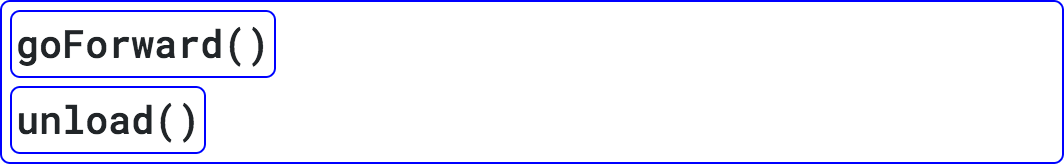
\includegraphics[width=\textwidth]{gfx/exercises-program-1.png}
    \caption{Musterlösung zu Aufgabe 1}
  \end{subfigure}\hfill
  \caption{Welt und Musterlösung zu Aufgabe 1}
\end{figure}

\pagebreak

\section{Aufgabe 2}
\label{sec:exercises:2}

Dieses Mal musst Du die Fracht erst aufladen. Dein Weg enthält außerdem eine Kurve. Reihe mehrere Befehle aneinander, um die Aufgabe zu lösen.

\begin{description}[noitemsep]
  \item[Welt wählen:] Welt B
  \item[Du brauchst:] Befehle
  \item[Video:] \url{https://vimeo.com/315545287} (Passwort: trucklino)
\end{description}

\begin{figure}[H]
  \begin{subfigure}[b]{0.40\textwidth}
    \includegraphics[width=\textwidth]{gfx/exercises-world-b.png}
    \caption{Welt B}
  \end{subfigure}\hfill
  \begin{subfigure}[b]{0.40\textwidth}
    \includegraphics[width=\textwidth]{gfx/exercises-program-2.png}
    \caption{Musterlösung zu Aufgabe 2}
  \end{subfigure}\hfill
  \caption{Welt und Musterlösung zu Aufgabe 2}
\end{figure}

\pagebreak

\section{Aufgabe 3}
\label{sec:exercises:3}

Erkennst Du das Muster? Wenn Du Deine Befehle in einer Prozedur verpackst, bleibt Dein Programm kurz und übersichtlich.

\begin{description}[noitemsep]
  \item[Welt wählen:] Welt C
  \item[Du brauchst:] Befehle, eigene Prozeduren
  \item[Video:] \url{https://vimeo.com/315545769} (Passwort: trucklino)
\end{description}

\begin{figure}[H]
  \begin{subfigure}[b]{0.40\textwidth}
    \includegraphics[width=\textwidth]{gfx/exercises-world-c.png}
    \caption{Welt C}
  \end{subfigure}\hfill
  \begin{subfigure}[b]{0.40\textwidth}
    \includegraphics[width=\textwidth]{gfx/exercises-program-3.png}
    \caption{Musterlösung zu Aufgabe 3}
  \end{subfigure}\hfill
  \caption{Welt und Musterlösung zu Aufgabe 3}
\end{figure}

\pagebreak

\section{Aufgabe 4}
\label{sec:exercises:4}

Deine Prozedur kannst Du auch in einer Zählerschleife mehrmals hintereinander ausführen.

\begin{description}[noitemsep]
  \item[Welt wählen:] Welt C
  \item[Du brauchst:] Befehle, eigene Prozeduren, Zählerschleife
  \item[Video:] \url{https://vimeo.com/315545858} (Passwort: trucklino)
\end{description}

\begin{figure}[H]
  \begin{subfigure}[b]{0.40\textwidth}
    \includegraphics[width=\textwidth]{gfx/exercises-world-c.png}
    \caption{Welt C}
  \end{subfigure}\hfill
  \begin{subfigure}[b]{0.40\textwidth}
    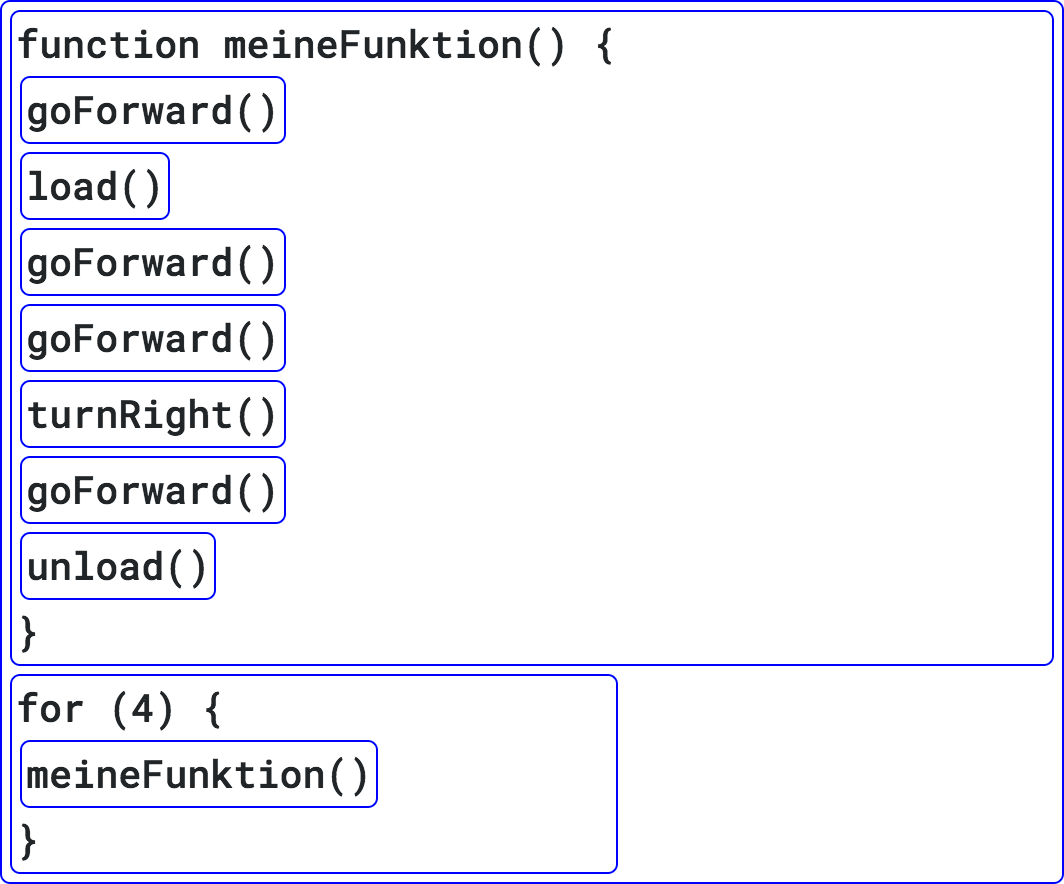
\includegraphics[width=\textwidth]{gfx/exercises-program-4.png}
    \caption{Musterlösung zu Aufgabe 4}
  \end{subfigure}\hfill
  \caption{Welt und Musterlösung zu Aufgabe 4}
\end{figure}

\pagebreak

\section{Aufgabe 5}
\label{sec:exercises:5}

Was passiert, wenn Du nicht weißt, wie oft Du Deine Prozedur ausführen musst? Benutze Sensoren und eine abweisende Schleife, um Deine Prozedur mehrmals auszuführen. Teste Dein Programm mit Welt B, C und D.

\begin{description}[noitemsep]
  \item[Welt wählen:] Welt B, Welt C, Welt D
  \item[Du brauchst:] Befehle, eigene Prozeduren, Sensoren, abweisende Schleife
  \item[Video:] \url{https://vimeo.com/315545914} (Passwort: trucklino)
\end{description}

\begin{figure}[H]
  \begin{subfigure}[b]{0.40\textwidth}
    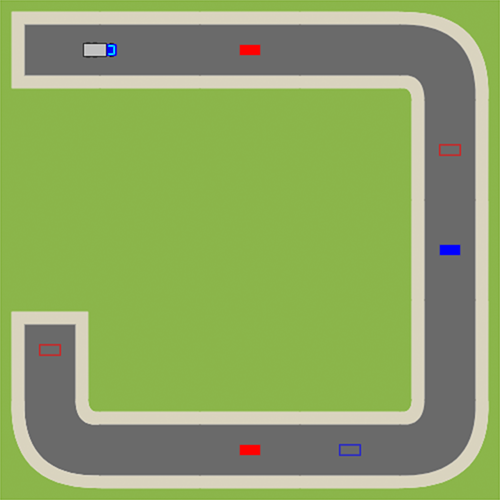
\includegraphics[width=\textwidth]{gfx/exercises-world-d.png}
    \caption{Welt D}
  \end{subfigure}\hfill
  \begin{subfigure}[b]{0.40\textwidth}
    \includegraphics[width=\textwidth]{gfx/exercises-program-5.png}
    \caption{Musterlösung zu Aufgabe 5}
  \end{subfigure}\hfill
  \caption{Welt und Musterlösung zu Aufgabe 5}
\end{figure}

\pagebreak

\section{Aufgabe 6}
\label{sec:exercises:6}

Statt einer abweisenden Schleife kannst Du auch Rekursion benutzen. Benutze eine Verzweigung, um Deine Prozedur im richtigen Moment zu verlassen.

\begin{description}[noitemsep]
  \item[Welt wählen:] Welt B, Welt C, Welt D
  \item[Du brauchst:] Befehle, eigene Prozeduren, Sensoren, Verzweigungen
  \item[Video:] \url{https://vimeo.com/315545989} (Passwort: trucklino)
\end{description}

\begin{figure}[H]
  \begin{subfigure}[b]{0.40\textwidth}
    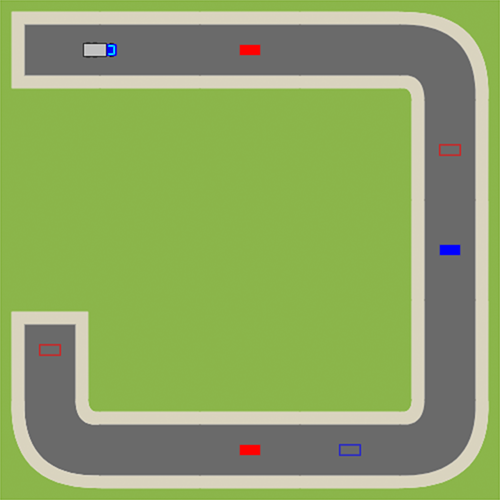
\includegraphics[width=\textwidth]{gfx/exercises-world-d.png}
    \caption{Welt D}
  \end{subfigure}\hfill
  \begin{subfigure}[b]{0.40\textwidth}
    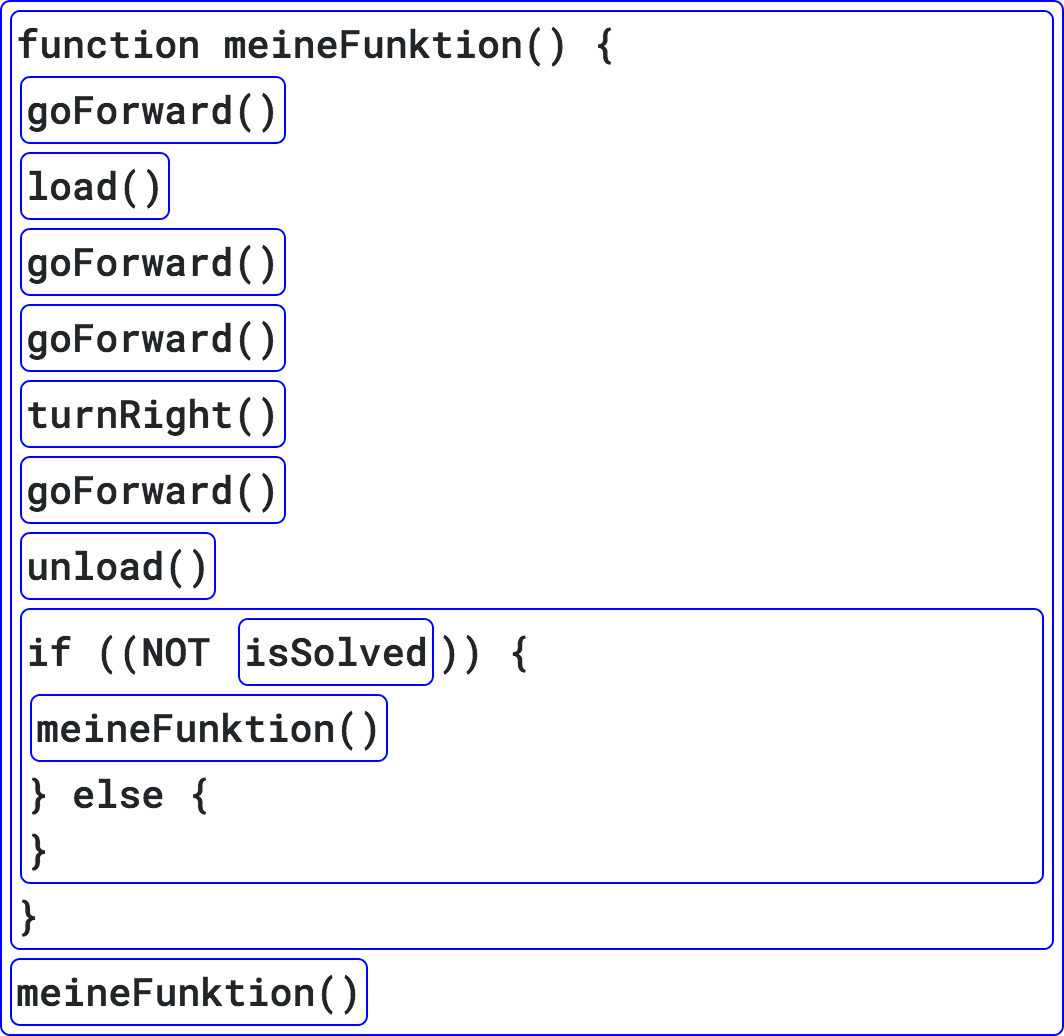
\includegraphics[width=\textwidth]{gfx/exercises-program-6.png}
    \caption{Musterlösung zu Aufgabe 6}
  \end{subfigure}\hfill
  \caption{Welt und Musterlösung zu Aufgabe 6}
\end{figure}

\pagebreak

\section{Aufgabe 7}
\label{sec:exercises:7}

Baue eine eigene Prozedur, die nicht nur geradeaus, sondern auch durch Kurven fahren kann. Deine Prozedur kannst Du solange aufrufen, bis Du am Ziel bist. Benutze dafür entweder eine abweisende Schleife oder Rekursion. Wenn Dein Programm mit Welt E funktioniert, probiere auch Welt F aus.

\begin{description}[noitemsep]
  \item[Welt wählen:] Welt E, Welt F
  \item[Du brauchst:] Befehle, eigene Prozeduren, Sensoren, Verzweigungen, abweisende Schleife (optional)
  \item[Video:] \url{https://vimeo.com/315546116} (Passwort: trucklino)
\end{description}

\begin{figure}[H]
  \begin{subfigure}[b]{0.40\textwidth}
    \includegraphics[width=\textwidth]{gfx/exercises-world-e.png}
    \caption{Welt E}
  \end{subfigure}\hfill
  \begin{subfigure}[b]{0.40\textwidth}
    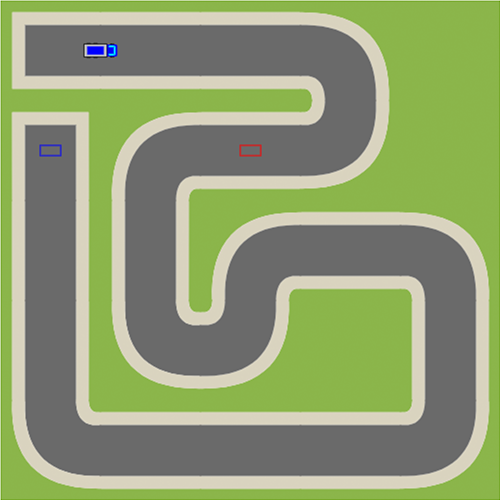
\includegraphics[width=\textwidth]{gfx/exercises-world-f.png}
    \caption{Welt F}
  \end{subfigure}\hfill
  \vspace{0.5cm}
  \begin{subfigure}[b]{0.40\textwidth}
    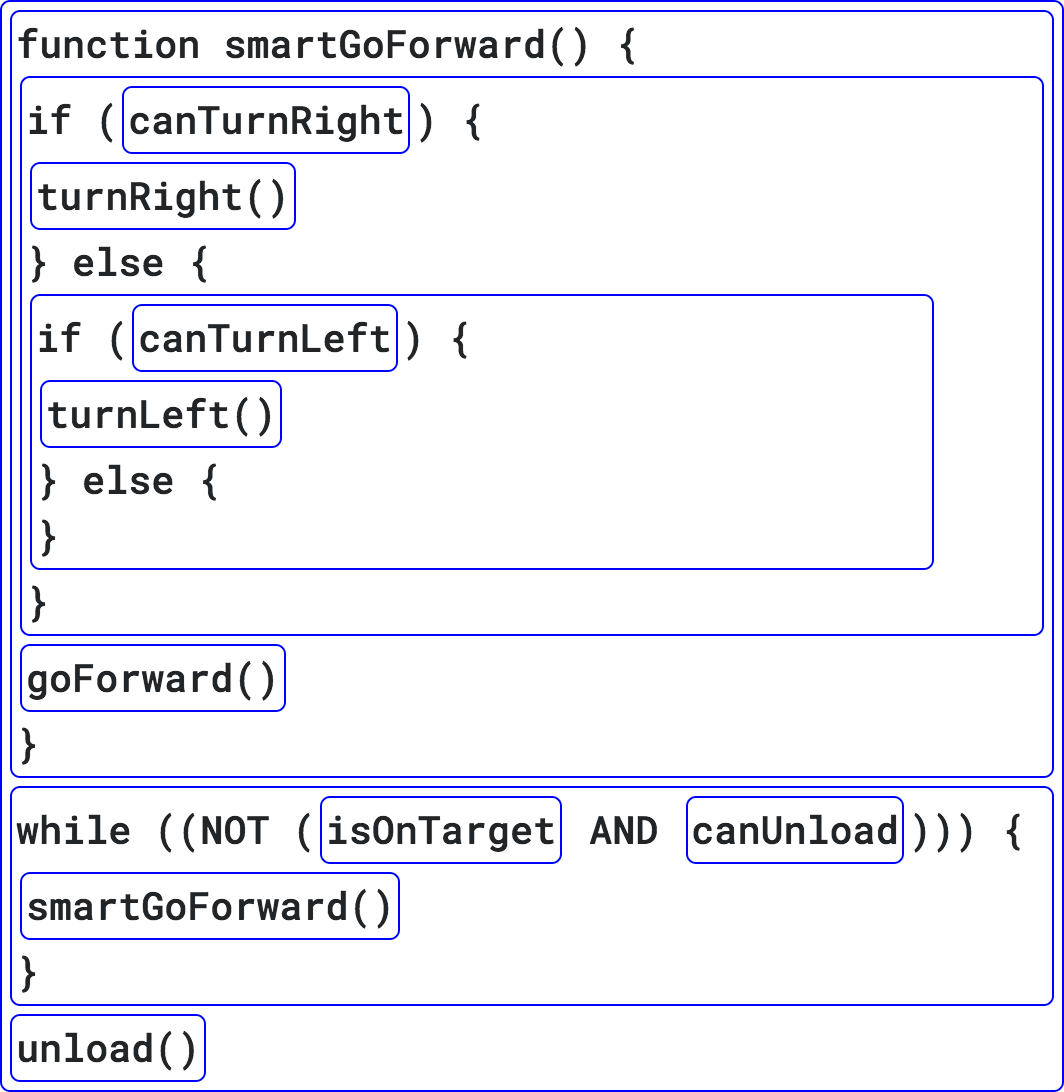
\includegraphics[width=\textwidth]{gfx/exercises-program-7.png}
    \caption{Musterlösung zu Aufgabe 7}
  \end{subfigure}\hfill
  \caption{Welten und Musterlösung zu Aufgabe 7}
\end{figure}

\pagebreak

\section{Aufgabe 8}
\label{sec:exercises:8}

Auf dem Weg sind nun einige Ampeln. Baue Dir eine zusätzliche Prozedur, die wartet, bis es grün wird.

\begin{description}[noitemsep]
  \item[Welt wählen:] Welt G
  \item[Du brauchst:] Befehle, eigene Prozeduren, Sensoren, Verzweigungen, abweisende Schleife (optional)
  \item[Video:] \url{https://vimeo.com/315546210} (Passwort: trucklino)
\end{description}

\begin{figure}[H]
  \begin{subfigure}[b]{0.40\textwidth}
    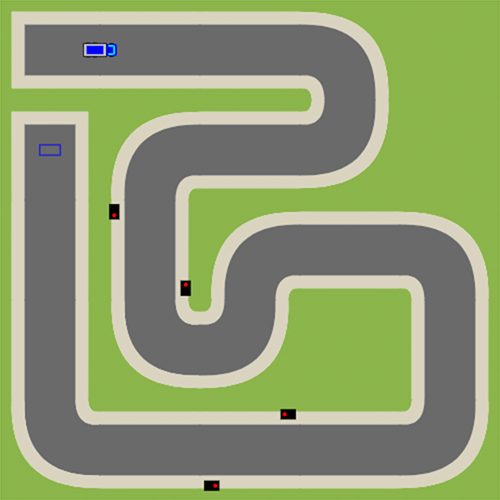
\includegraphics[width=\textwidth]{gfx/exercises-world-g.png}
    \caption{Welt G}
  \end{subfigure}\hfill
  \begin{subfigure}[b]{0.40\textwidth}
    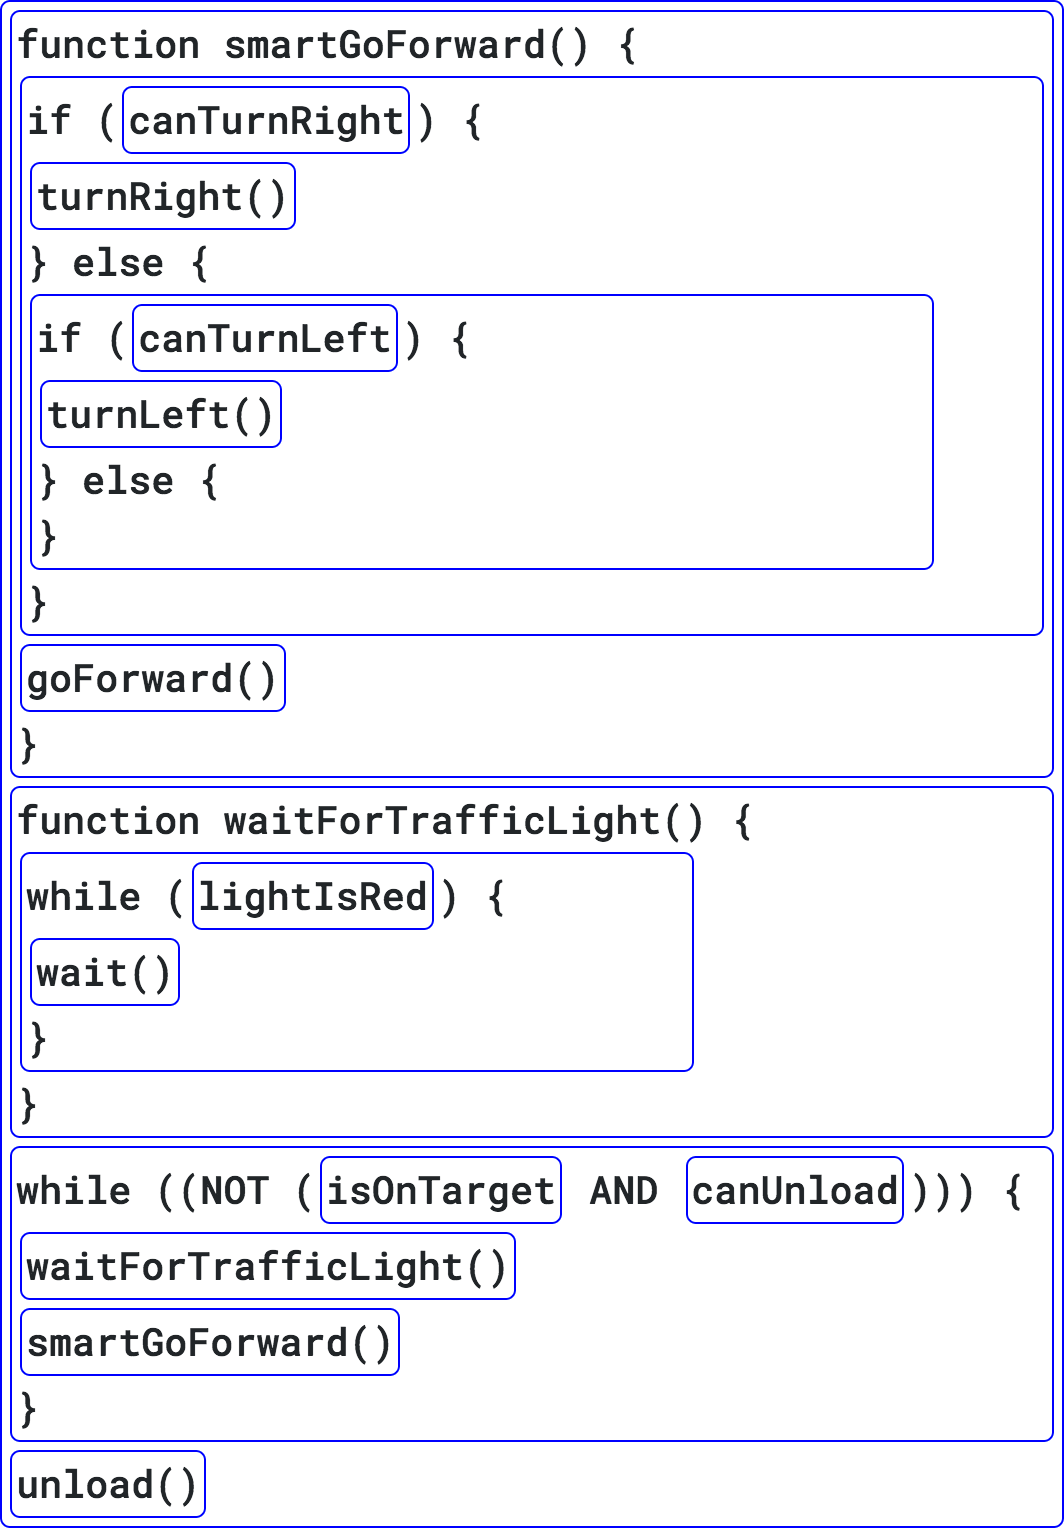
\includegraphics[width=\textwidth]{gfx/exercises-program-8.png}
    \caption{Musterlösung zu Aufgabe 8}
  \end{subfigure}\hfill
  \caption{Welt und Musterlösung zu Aufgabe 8}
\end{figure}

%%************************************************
% CD-ROM
%************************************************
\chapter{CD-ROM}
\label{sec:cd-rom}

Alle auf der beigefügten CD-ROM enthaltenen Daten sind auch im BlattWerkzeug-Git-Repository unter \url{http://blattwerkzeug.de/forward/git-repository} verfügbar.


% \listoffigures
% \cleardoublepage

% \listoftables
% \cleardoublepage

%************************************************
% Declaration
%************************************************
% \pdfbookmark[0]{Eidesstattliche Erklärung}{Eidesstattliche Erklärung}
\chapter{Eidesstattliche Erklärung}
\label{sec:declaration}
\thispagestyle{empty}

Ich erkläre hiermit an Eides statt, dass ich die vorliegende Arbeit selbstständig und ohne Benutzung anderer als der angegebenen Hilfsmittel angefertigt habe; die aus fremden Quellen direkt oder indirekt übernommenen Gedanken sind als solche kenntlich gemacht. Die Arbeit wurde bisher in ähnlicher Form keiner anderen Prüfungskommission vorgelegt und auch nicht veröffentlicht.

\bigskip
\bigskip
\bigskip
\bigskip

\begin{multicols}{2}
    \raggedright
    \thesisUniversityCity, \thesisDate

    \raggedleft
    \thesisAuthor
\end{multicols}

\cleardoublepage
